\documentclass[11pt]{article}

\usepackage[preprint]{neurips_2025}
\usepackage[T1]{fontenc}
\usepackage[utf8]{inputenc}
\usepackage{lmodern}
\usepackage{mathtools}
\usepackage{amsthm}
\usepackage{hyperref}
\usepackage{cleveref}
\usepackage{url}
\usepackage{booktabs}
\usepackage{amsfonts}
\usepackage{microtype}
\usepackage{xcolor}
\usepackage{graphicx}
\usepackage{caption}
\usepackage{amsmath,amssymb}
\usepackage{enumitem}

\captionsetup{font=small,labelfont=bf}
\setlist[itemize]{leftmargin=1.1em, itemsep=0.2em, topsep=0.35em}
\setlist[enumerate]{leftmargin=1.25em, itemsep=0.2em, topsep=0.35em}
\hypersetup{colorlinks=true,linkcolor=black,citecolor=black,urlcolor=neuripsblue}

\newcommand{\appendixsnapshot}{%
{\small
\setlength{\tabcolsep}{5pt}
\renewcommand{\arraystretch}{1.06}
\sloppy
% Auto-generated paper appendix fragment.
\subsection*{Appendix Snapshot}
This appendix summarizes the pooled OpenAI GPT and Anthropic Claude benchmark over 6912 scored responses. The full machine-generated statistics remain available separately in \texttt{appendix\_snapshot\_full.tex}.
The pooled fit yields $\alpha=3.262$ with 95\% interval $[2.959, 3.558]$ and $\beta=0.092$ with interval $[-0.279, 0.460]$.

\subsubsection*{Top-Line Summary}
\begin{center}
\begin{tabular}{lr}
\toprule
Metric & Value \\
\midrule
Usable evaluations & 6912 \\
Mean $d_{phys}$ & 0.408 \\
Median $d_{phys}$ & 0.302 \\
Exact-correct rate & 0.345 \\
$d_{phys} \ge 0.5$ rate & 0.403 \\
Full-error rate & 0.274 \\
Best model & Claude Opus 4.1 \\
Weakest model & GPT-4o mini \\
\bottomrule
\end{tabular}
\end{center}

\subsubsection*{Model Ranking}
\begin{center}
\begin{tabular}{lrrrr}
\toprule
Model & Mean & 95\% CI & Exact & Full \\
\midrule
Claude Opus 4.1 & 0.138 & [0.116, 0.160] & 0.582 & 0.082 \\
GPT-5.4 & 0.329 & [0.301, 0.357] & 0.430 & 0.195 \\
GPT-5.2 & 0.368 & [0.338, 0.397] & 0.380 & 0.249 \\
GPT-5.4 mini & 0.394 & [0.364, 0.424] & 0.372 & 0.267 \\
GPT-4.1 & 0.442 & [0.412, 0.471] & 0.311 & 0.293 \\
Claude Sonnet 4 & 0.450 & [0.419, 0.481] & 0.305 & 0.332 \\
GPT-4.1 mini & 0.478 & [0.449, 0.507] & 0.285 & 0.311 \\
GPT-5.1 & 0.501 & [0.472, 0.531] & 0.260 & 0.355 \\
GPT-4o mini & 0.570 & [0.543, 0.598] & 0.177 & 0.378 \\
\bottomrule
\end{tabular}
\end{center}

\subsubsection*{Depth and Category Breakdown}
\noindent\begin{minipage}[t]{0.42\linewidth}
\centering
\textbf{By depth}\\[0.25em]
\begin{tabular}{rrrr}
\toprule
Depth & Mean & Exact & Full \\
\midrule
1 & 0.403 & 0.349 & 0.275 \\
2 & 0.415 & 0.340 & 0.275 \\
4 & 0.405 & 0.345 & 0.271 \\
\bottomrule
\end{tabular}
\end{minipage}\hfill
\begin{minipage}[t]{0.54\linewidth}
\centering
\textbf{By category}\\[0.25em]
\begin{tabular}{lrrr}
\toprule
Category & Mean & Exact & Full \\
\midrule
Circuit & 0.657 & 0.213 & 0.476 \\
Measurement & 0.520 & 0.284 & 0.417 \\
Operator & 0.258 & 0.078 & 0.006 \\
Entanglement & 0.196 & 0.804 & 0.196 \\
\bottomrule
\end{tabular}
\end{minipage}

\subsubsection*{Model-by-Category Means}
\begin{center}
\begin{tabular}{lrrrr}
\toprule
Model & Circuit & Measurement & Operator & Entanglement \\
\midrule
Claude Opus 4.1 & 0.367 & 0.068 & 0.117 & 0.000 \\
GPT-5.4 & 0.592 & 0.509 & 0.215 & 0.000 \\
GPT-5.2 & 0.659 & 0.587 & 0.224 & 0.000 \\
GPT-5.4 mini & 0.721 & 0.586 & 0.270 & 0.000 \\
GPT-4.1 & 0.697 & 0.552 & 0.283 & 0.234 \\
Claude Sonnet 4 & 0.658 & 0.432 & 0.258 & 0.453 \\
GPT-4.1 mini & 0.728 & 0.635 & 0.308 & 0.240 \\
GPT-5.1 & 0.707 & 0.602 & 0.302 & 0.396 \\
GPT-4o mini & 0.786 & 0.711 & 0.347 & 0.438 \\
\bottomrule
\end{tabular}
\end{center}

\subsubsection*{Anthropic Repair Ablation}
After fixing output extraction to score the final machine-readable literal even when it is preceded by explanatory text, we ran a separate 32-task Claude repair ablation using Claude Sonnet 4 and Claude Opus 4.1 at depth 4 with a five-minute per-prompt budget.

\begin{center}
\begin{tabular}{lrrr}
\toprule
Mode & Solve rate & Mean solve time & Median solve time \\
\midrule
One-shot & 0.594 & 6.114 s & 6.383 s \\
Self-retry & 0.812 & 7.506 s & 6.806 s \\
Verifier feedback & 0.938 & 11.258 s & 7.114 s \\
\bottomrule
\end{tabular}
\end{center}

\noindent Category solve rates under the same Claude repair ablation were:
\begin{center}
\begin{tabular}{lccc}
\toprule
Category & One-shot & Self-retry & Verifier feedback \\
\midrule
Circuit & 0.625 & 0.625 & 0.875 \\
Measurement & 0.625 & 0.875 & 0.875 \\
Operator & 0.500 & 0.750 & 1.000 \\
Entanglement & 0.625 & 1.000 & 1.000 \\
\bottomrule
\end{tabular}
\end{center}

\noindent By model, Claude Opus 4.1 solved all 32 subset prompts in every repair mode, while Claude Sonnet 4 improved from 0.188 one-shot solve rate to 0.625 with self-retry and 0.875 with verifier feedback.

}%
}

\title{QuantumPhysEval: Measuring Quantum Hallucinations in LLMs}
\author{%
  Manish Bhatt\thanks{Corresponding author: \texttt{manish.bhatt13212@gmail.com}.}\thanks{This work was conducted independently and does not necessarily reflect the views, policies, or endorsements of OWASP or any current or former employer.}\\
  OWASP
}
\date{}

\begin{document}
\maketitle

\begin{abstract}
This paper presents QuantumPhysEval, a benchmark developed to measure whether large language models produce physically inconsistent yet superficially plausible answers on elementary quantum-mechanical tasks. QuantumPhysEval evaluates model behavior in four task families central to introductory quantum reasoning: circuit evolution, operator composition, measurement prediction, and entanglement classification. Because the benchmark is built from analytically generated small-system quantum problems, it supports exact self-generated ground truth and fully automated scoring with bounded normalized physics-error metrics. Through a case study involving seven OpenAI GPT-family models and two Anthropic Claude-family models across three prompted reasoning-depth settings, QuantumPhysEval identifies clear reliability gaps and offers practical insight into where those models fail. In the pooled 2-qubit analysis of 6{,}912 evaluations, benchmark error decreases strongly with a model-size proxy, with fitted exponent $\alpha=3.262$ and bootstrap 95\% interval $[2.959, 3.558]$, while prompted reasoning depth shows only a weak effect with $\beta=0.092$ and interval $[-0.279, 0.460]$. In a matched 4-qubit stress test over the same model sets, mean error rises from 0.408 to 0.533, with the largest degradations in circuit evolution ($+0.185$) and measurement prediction ($+0.188$). In a completed Anthropic 2q$\rightarrow$4q$\rightarrow$8q complexity ladder, mean error rises monotonically from 0.294 to 0.437 to 0.542, while circuit evolution and measurement prediction degrade by $+0.388$ and $+0.510$ from 2 to 8 qubits and operator composition remains flat as a control. A completed GPT 2q$\rightarrow$4q$\rightarrow$8q ladder over 5{,}374 usable 8-qubit responses shows the same pattern, with family mean error rising from 0.440 to 0.561 to 0.682, circuit evolution and measurement prediction saturating at 1.000 and 0.999 mean error, and operator composition remaining much lower at 0.277. A separate 64-task OpenAI repair ablation shows that one-shot solving reaches 0.422 solved fraction, blind self-retry reaches 0.609, and verifier-guided retry reaches 0.688, with nearly all gains saturating within the first 30 seconds. After adding robust final-literal extraction for mixed prose and code-block outputs, a matched 32-task Claude repair ablation yields 0.594 one-shot solve rate, 0.813 self-retry, and 0.938 verifier-feedback solve rate.
\end{abstract}

\section{Introduction}
Large Language Models (LLMs) have shown strong performance on many reasoning and coding tasks, but there are still relatively few benchmarks designed to measure whether their outputs remain faithful to exact scientific structure. In quantum information settings, this matters because correct answers must satisfy sharply defined physical constraints such as normalization, unitarity, linear state evolution, and the Born rule. An answer can therefore look polished and plausible while still being physically wrong.

In this work, we identify one major reliability risk for language models in this domain: \emph{quantum hallucination}, which we define as a model output that is syntactically plausible but inconsistent with exact quantum-mechanical ground truth or with basic physical constraints. To measure this risk, we develop QuantumPhysEval, an evaluation suite intended to integrate directly into model testing workflows in the same way that safety and robustness benchmarks are used in other domains.

\subsection{QuantumPhysEval Approach}
QuantumPhysEval's overall approach is straightforward. First, we construct benchmark prompts from analytically generated quantum tasks so that exact targets are known by construction. Second, we score model outputs using bounded physics-grounded error metrics rather than subjective grading. Third, we apply the resulting benchmark to multiple model families and prompted depth settings in order to understand which kinds of quantum tasks remain difficult and whether stronger models reduce those errors. The primary case study uses exact 2-qubit tasks, a matched 4-qubit stress test measures how reliability changes as the state space expands, and a completed Anthropic 8-qubit ladder probes whether the same trend continues once the state vector grows to 256 amplitudes.

This benchmark is designed to be useful in practice. Because test generation, target generation, and evaluation are automated, the suite can be rerun easily as models improve. Because it uses exact small-system simulation, every failure corresponds to a real physical inconsistency rather than a matter of interpretation.

\subsection{Main Contributions}
Overall, QuantumPhysEval makes the following contributions:
\begin{itemize}
\item \textbf{Exactness}: every test case has an exact self-generated quantum target derived analytically inside the harness.
\item \textbf{Breadth}: the benchmark covers four distinct quantum reasoning families: circuit evolution, operator composition, measurement prediction, and entanglement classification.
\item \textbf{Automation}: test generation, model querying, parsing, scoring, and scaling-law fitting are fully automated.
\item \textbf{Actionability}: in a pooled OpenAI GPT and Anthropic Claude case study, the benchmark identifies concrete reliability gaps and isolates the task families that drive them.
\item \textbf{Complexity scaling}: matched larger-qubit reruns show that error grows with Hilbert-space size and that the growth is concentrated in dynamics-heavy tasks rather than in the fixed control slice.
\end{itemize}

\section{Benchmark Construction}
\begin{figure}[tb]
\centering
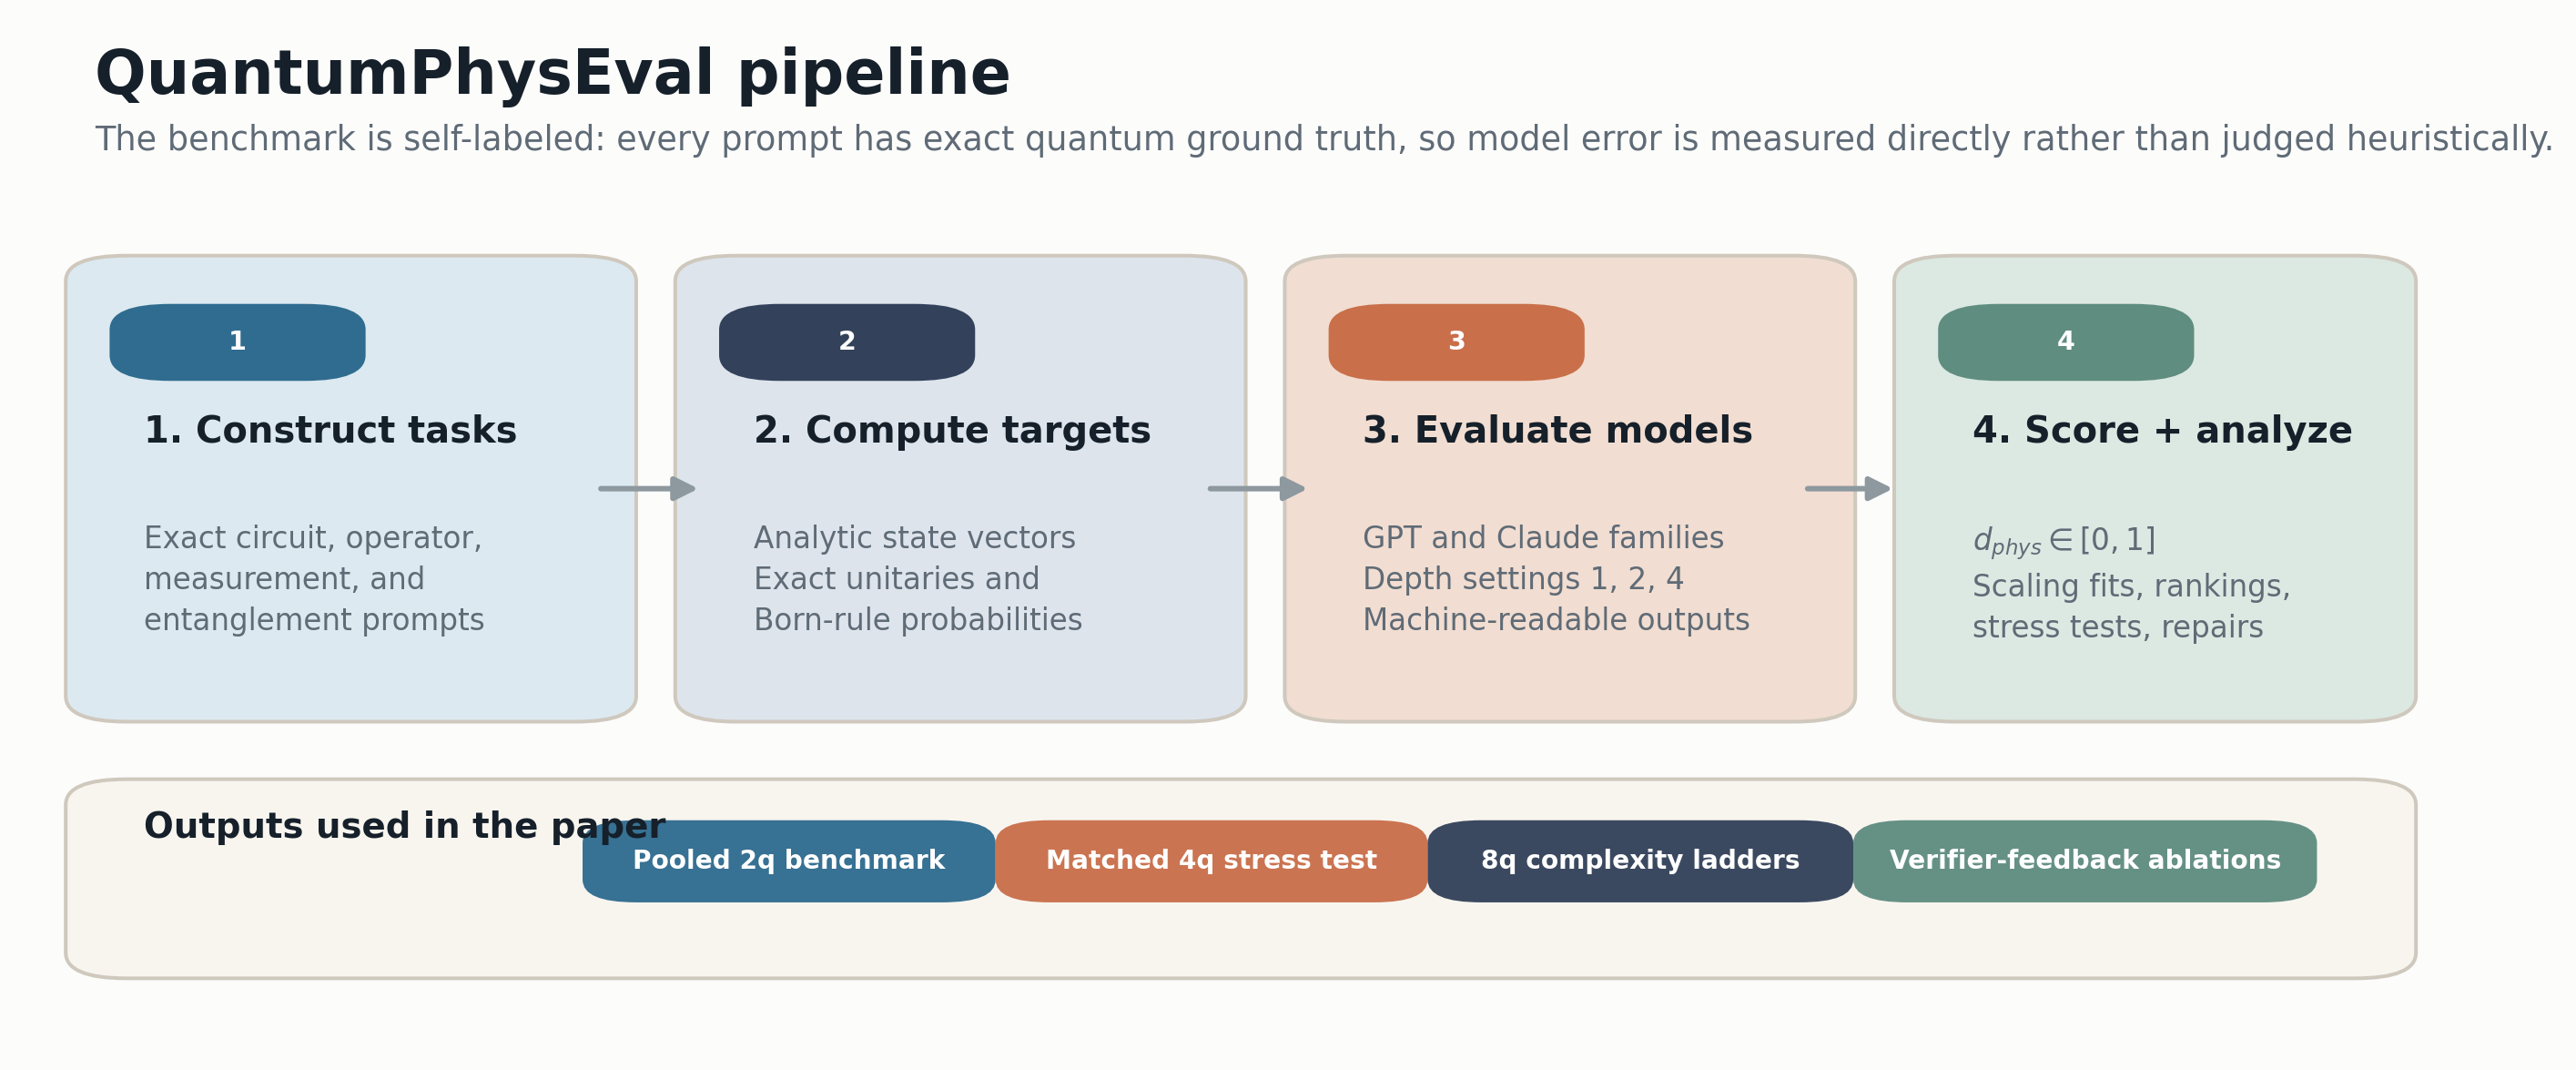
\includegraphics[width=\linewidth]{figures/quantumphys_eval_overview.png}
\caption{QuantumPhysEval benchmark overview. The pipeline is fully automated: exact small-system tasks are generated analytically, exact targets are computed by construction, model outputs are scored with a bounded physics-grounded error metric, and pooled trends are analyzed across model families and depth settings. The main case study uses 2-qubit tasks, a matched 4-qubit stress test measures immediate difficulty growth, and a completed Anthropic 8-qubit ladder extends the same logic to a larger state-space regime.}
\label{fig:overview}
\end{figure}

QuantumPhysEval contains four benchmark families:
\begin{itemize}
\item \textbf{Circuit evolution}: generate the final quantum state after a sampled gate sequence.
\item \textbf{Operator composition}: generate the exact one-qubit unitary corresponding to a sampled gate sequence.
\item \textbf{Measurement prediction}: generate the exact post-circuit measurement probabilities.
\item \textbf{Entanglement classification}: decide whether a provided two-qubit state is entangled.
\end{itemize}

\subsection{Constructing test cases}
All benchmark instances are generated analytically inside the evaluation harness. The gate library consists of single-qubit gates $\{I,H,X,Y,Z,S,T\}$ and two-qubit gates built from $\mathrm{CNOT}$ and $\mathrm{CZ}$. For circuit evolution and measurement prediction, the benchmark samples initial states and gate sequences and then computes exact outcomes. For operator composition, it samples one-qubit gate sequences and asks the model to return the corresponding unitary. For entanglement classification, it evaluates analytically specified product and entangled states. The primary pooled benchmark uses exact 2-qubit tasks; the matched stress test extends circuit evolution, measurement prediction, and entanglement classification to 4 qubits while keeping operator composition as a fixed one-qubit control task.

\subsection{Generating exact ground truth}
Ground truth is produced directly from quantum mechanics rather than external annotation. States and operators are computed by explicit matrix multiplication. Measurement targets are derived from exact Born-rule probabilities. Entanglement labels are attached by construction. This allows the benchmark to avoid noisy labels and to support exact automated evaluation. It also makes matched difficulty expansions possible, since the same harness can be rerun at larger qubit counts with exact targets.

\section{Methods}
Each model response is parsed into a structured object and scored with a bounded physics-grounded error metric $d_{phys}\in[0,1]$, where 0 indicates a correct response and 1 indicates a maximally bad or unparseable response under the benchmark metric.

\subsection{Scoring}
For circuit-evolution tasks, the predicted state is normalized, aligned up to global phase, and compared to the exact target using a combination of normalization penalty and one minus fidelity. For measurement tasks, negative values are clipped to zero, the output is renormalized, and the score combines total-variation distance with a normalization penalty. For operator-composition tasks, the score averages a unitarity penalty with a target-mismatch penalty based on normalized Frobenius norms. For entanglement classification, the score is 0 for an exact match and 1 otherwise.

To avoid confounding provider-specific formatting style with scientific correctness, the parser first attempts to read the full response as a literal and then falls back to extracting the final bracketed literal or boolean token when a model returns the answer after explanatory text or inside a code block.

\subsection{Case Study Protocol}
The pooled 2-qubit benchmark evaluates three completed runs: GPT-4-family models, GPT-5-family models, and a Claude-family run. Each model is tested at prompted reasoning-depth settings $D\in\{1,2,4\}$ with temperature fixed at 0.0. Across the three runs, the pooled 2-qubit evaluation contains 6{,}912 scored responses. To summarize aggregate behavior, we fit
\[
\mathbb{E}[d_{phys}] = k S^{-\alpha} D^{\beta},
\]
using a model-size proxy $S$ and log-linear least squares, with 2{,}000 bootstrap resamples for uncertainty estimation.

We then run a matched 4-qubit stress test on the same GPT and Claude model sets. This stress test adds another 6{,}912 scored responses and keeps the category schema fixed so that differences can be compared directly. Circuit evolution, measurement prediction, and entanglement classification are upgraded to 4 qubits, while operator composition remains a 1-qubit control slice.

To push the same question further, we also complete matched 8-qubit reruns. On the Anthropic side, Claude Sonnet 4 and Claude Opus 4.1 add 1{,}536 scored responses and create a clean 2q$\rightarrow$4q$\rightarrow$8q ladder for one provider family. On the GPT side, a full 8-qubit retry run yields 5{,}374 usable responses with only two residual API failures, which is sufficient to construct a parallel GPT 2q$\rightarrow$4q$\rightarrow$8q ladder rather than treating GPT 8q as merely provisional corroboration.

\subsection{Time-Budget Repair Ablation}
We also run a separate repair ablation designed to test whether the hardest failures are recoverable with additional interaction time. This ablation uses a strong-model subset consisting of \texttt{gpt-4.1}, \texttt{gpt-5.2}, \texttt{gpt-5.4-mini}, and \texttt{gpt-5.4}; depth 4 only; temperature 0.2; and four prompts per benchmark family, for 64 tasks total. Each prompt receives a five-minute wall-clock budget and is evaluated under three modes: \emph{one-shot}, \emph{self-retry}, and \emph{verifier feedback}.

\section{Results}
\subsection{Top-Level Findings}
The pooled mean normalized error is 0.408, with median 0.302. Exact-correct outputs occur on 34.5\% of samples, while 27.4\% of samples are effectively full-error failures. QuantumPhysEval is therefore measuring a substantial reliability gap rather than just small calibration drift.

\begin{table}[t]
\centering
\caption{Mean normalized physics error by model in the pooled case study. Lower is better.}
\label{tab:model-ranking}
\begin{tabular}{lr}
\toprule
Model & Mean $d_{phys}$ \\
\midrule
Claude Opus 4.1 & 0.138 \\
\texttt{gpt-5.4} & 0.329 \\
\texttt{gpt-5.2} & 0.368 \\
\texttt{gpt-5.4-mini} & 0.394 \\
\texttt{gpt-4.1} & 0.442 \\
Claude Sonnet 4 & 0.450 \\
\texttt{gpt-4.1-mini} & 0.478 \\
\texttt{gpt-5.1} & 0.501 \\
\texttt{gpt-4o-mini} & 0.570 \\
\bottomrule
\end{tabular}
\end{table}

\begin{figure}[tb]
\centering
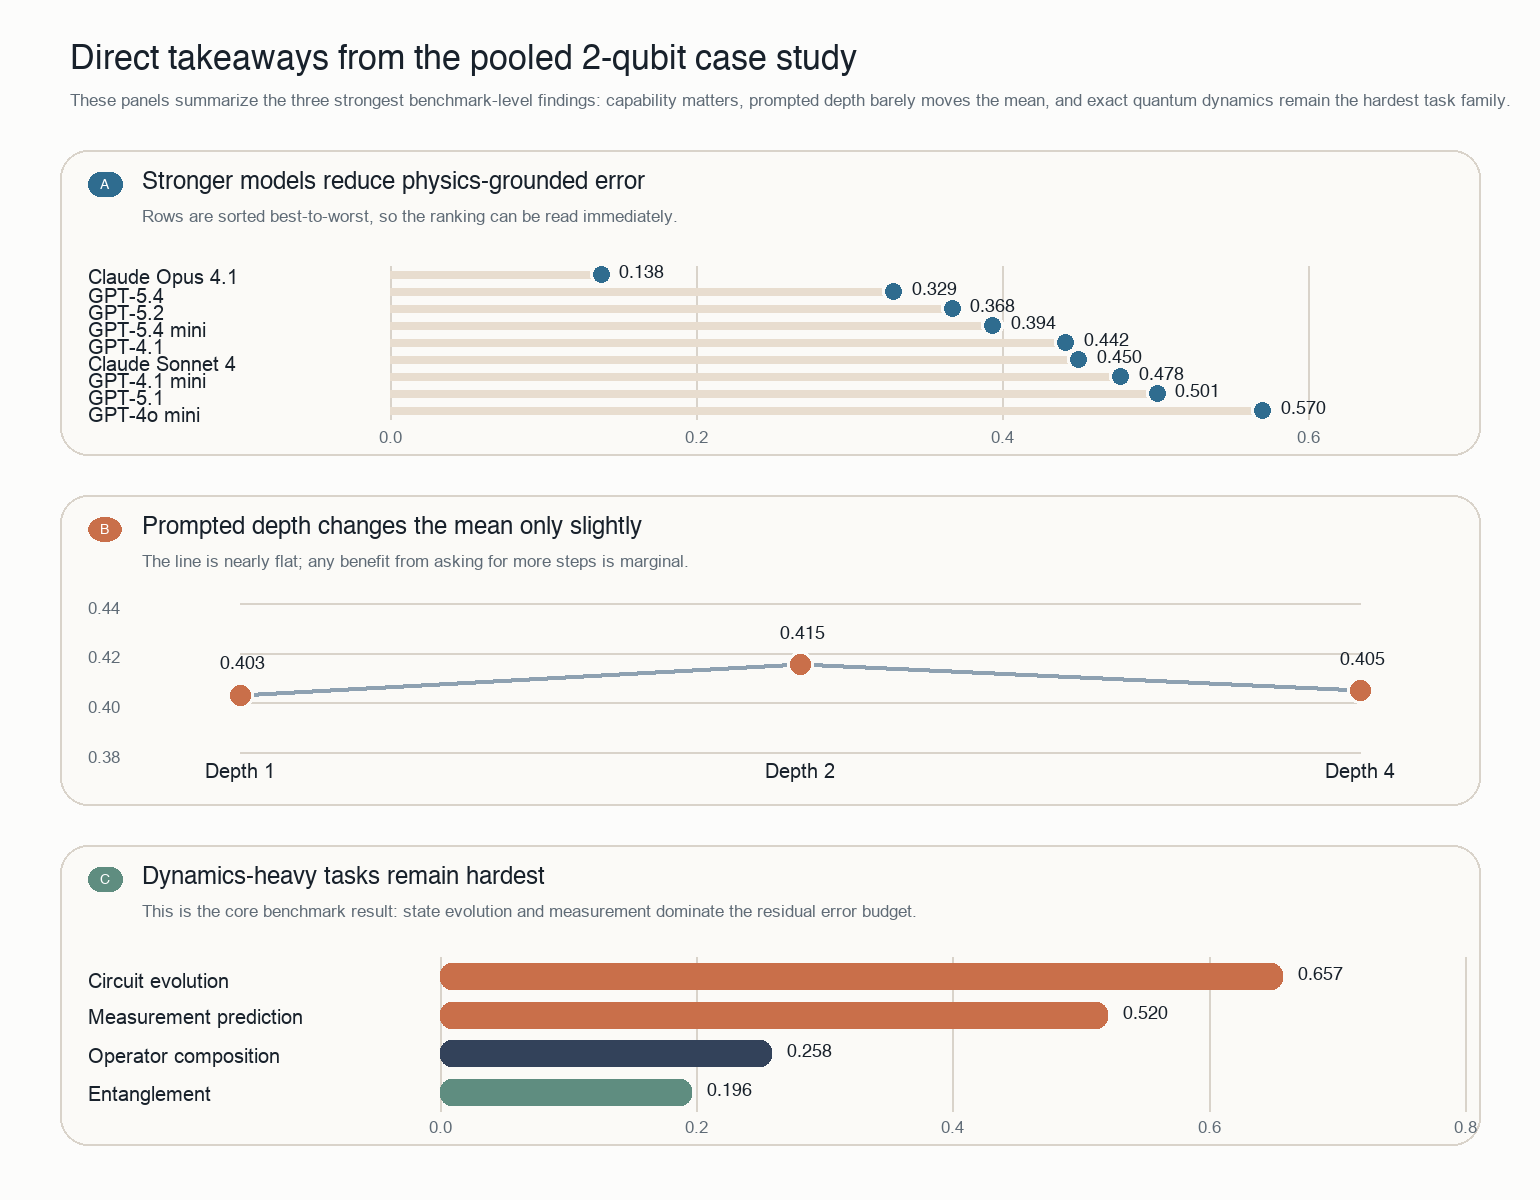
\includegraphics[width=\linewidth]{figures/combined_quantum_takeaways.png}
\caption{Direct takeaways from the pooled OpenAI GPT and Anthropic Claude case study. Left: stronger models reduce physics-grounded error. Middle: more prompted reasoning depth changes the result only slightly. Right: the hardest residual failures remain circuit evolution and measurement prediction.}
\label{fig:takeaways}
\end{figure}

\subsection{Scaling Behavior}
The strongest quantitative pattern in the pooled analysis is the size effect. Fitting the pooled data yields $\alpha=3.262$ with bootstrap 95\% CI $[2.959, 3.558]$. The prompted reasoning-depth effect is much weaker, with $\beta=0.092$ and bootstrap 95\% CI $[-0.279, 0.460]$. Average error at depth 4 is 0.405, compared with 0.403 at depth 1 and 0.415 at depth 2.

\begin{figure}[tb]
\centering
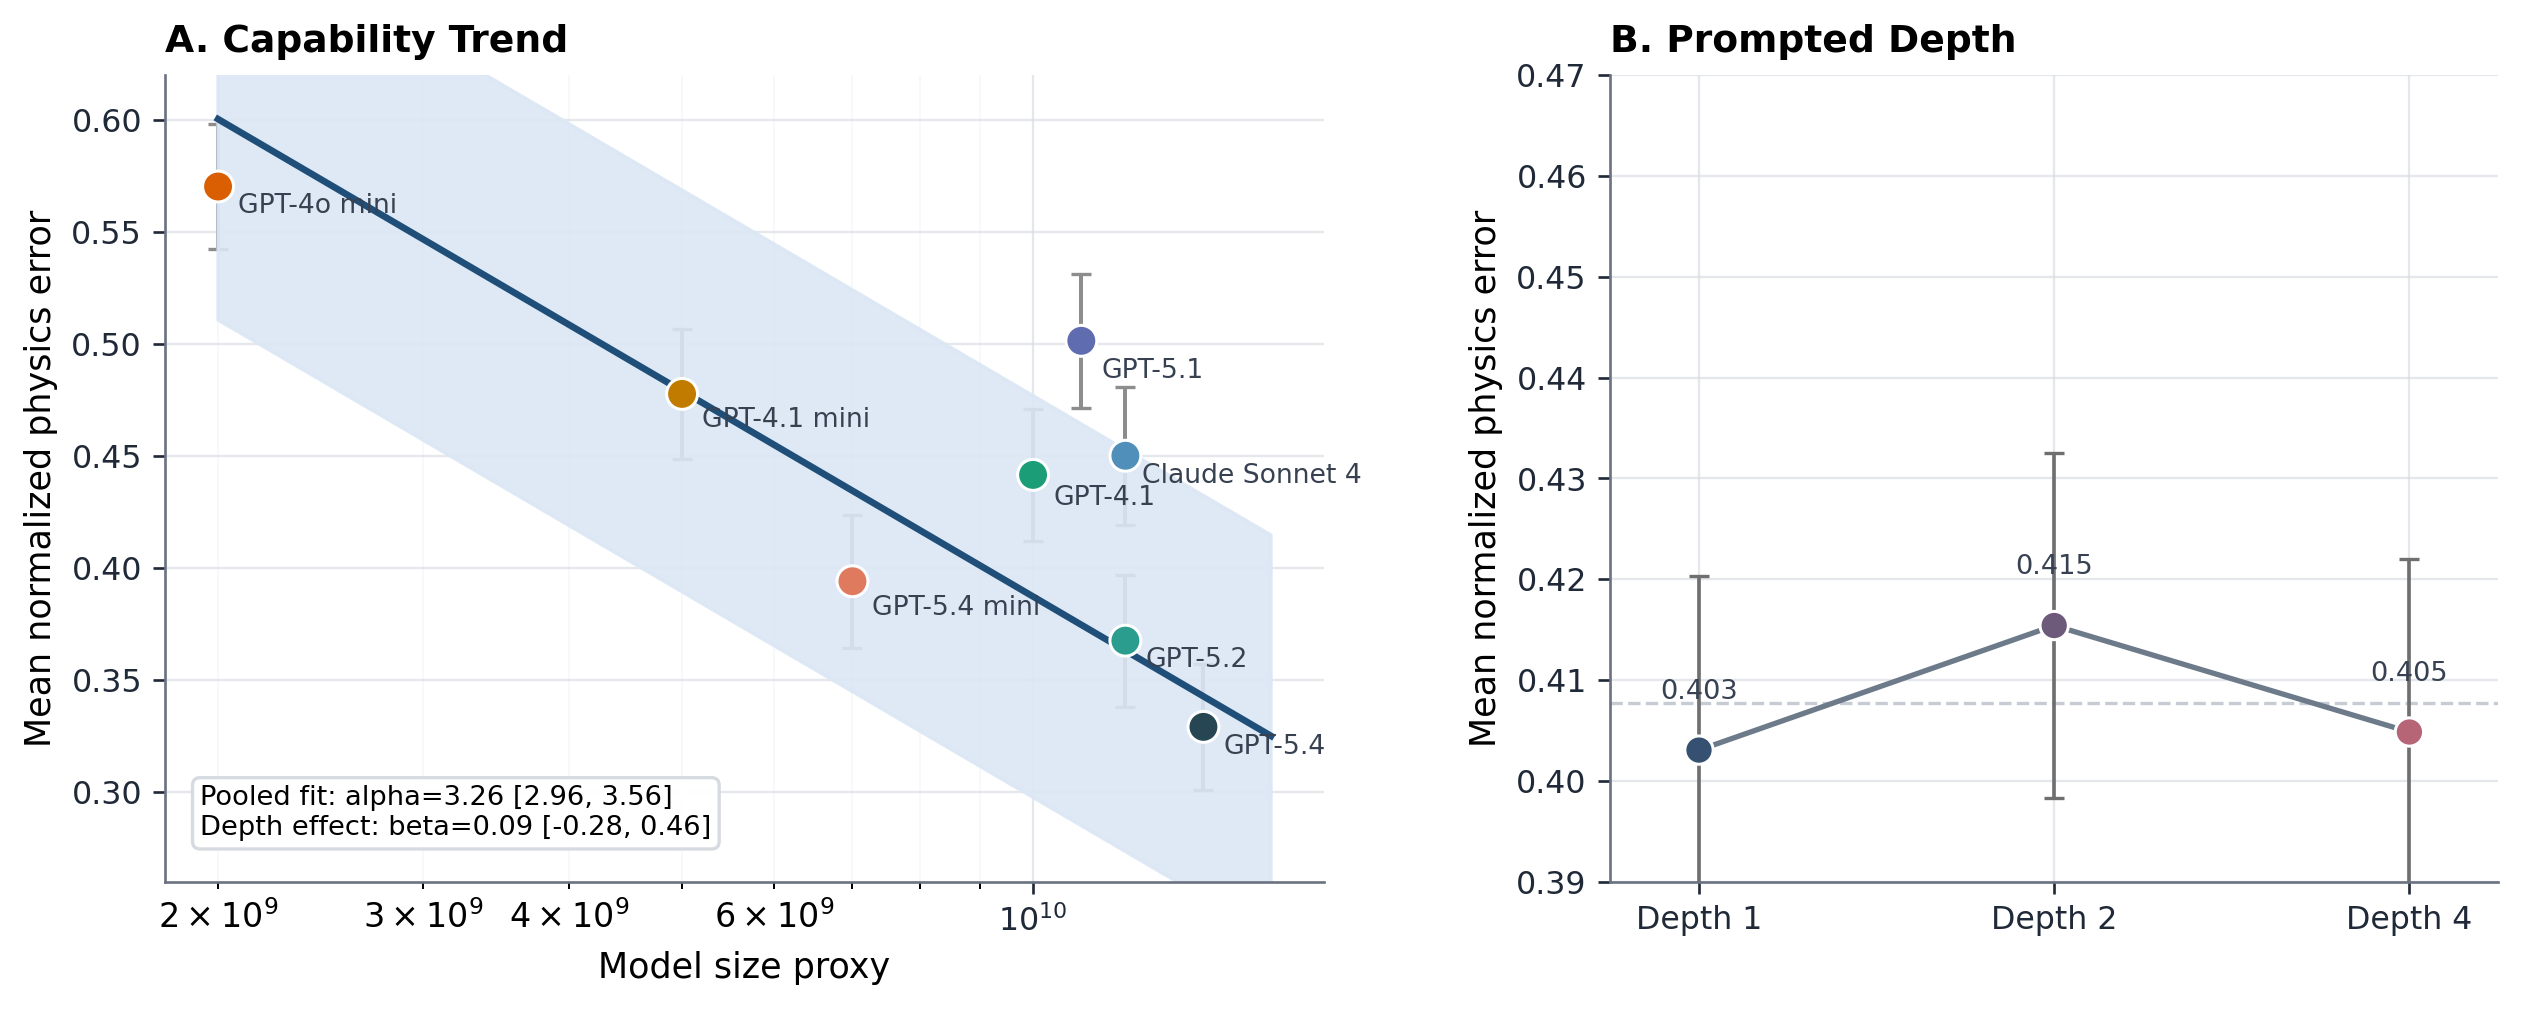
\includegraphics[width=\linewidth]{figures/combined_quantum_scaling.png}
\caption{Pooled scaling behavior in the 2-qubit case study. Left: benchmark error falls as the model-capability proxy increases, with the fitted size effect shown directly on the pooled data. Right: prompted depth conditions remain tightly clustered, consistent with the weak fitted depth effect.}
\label{fig:pooled-scaling}
\end{figure}

\subsection{Benchmark-Family Findings}
Benchmark-family differences are pronounced. In the pooled run, category means are 0.657 for circuit evolution, 0.520 for measurement prediction, 0.258 for operator composition, and 0.196 for entanglement classification. The dominant residual risks therefore arise in tasks that require exact quantum dynamics.

\begin{figure}[tb]
\centering
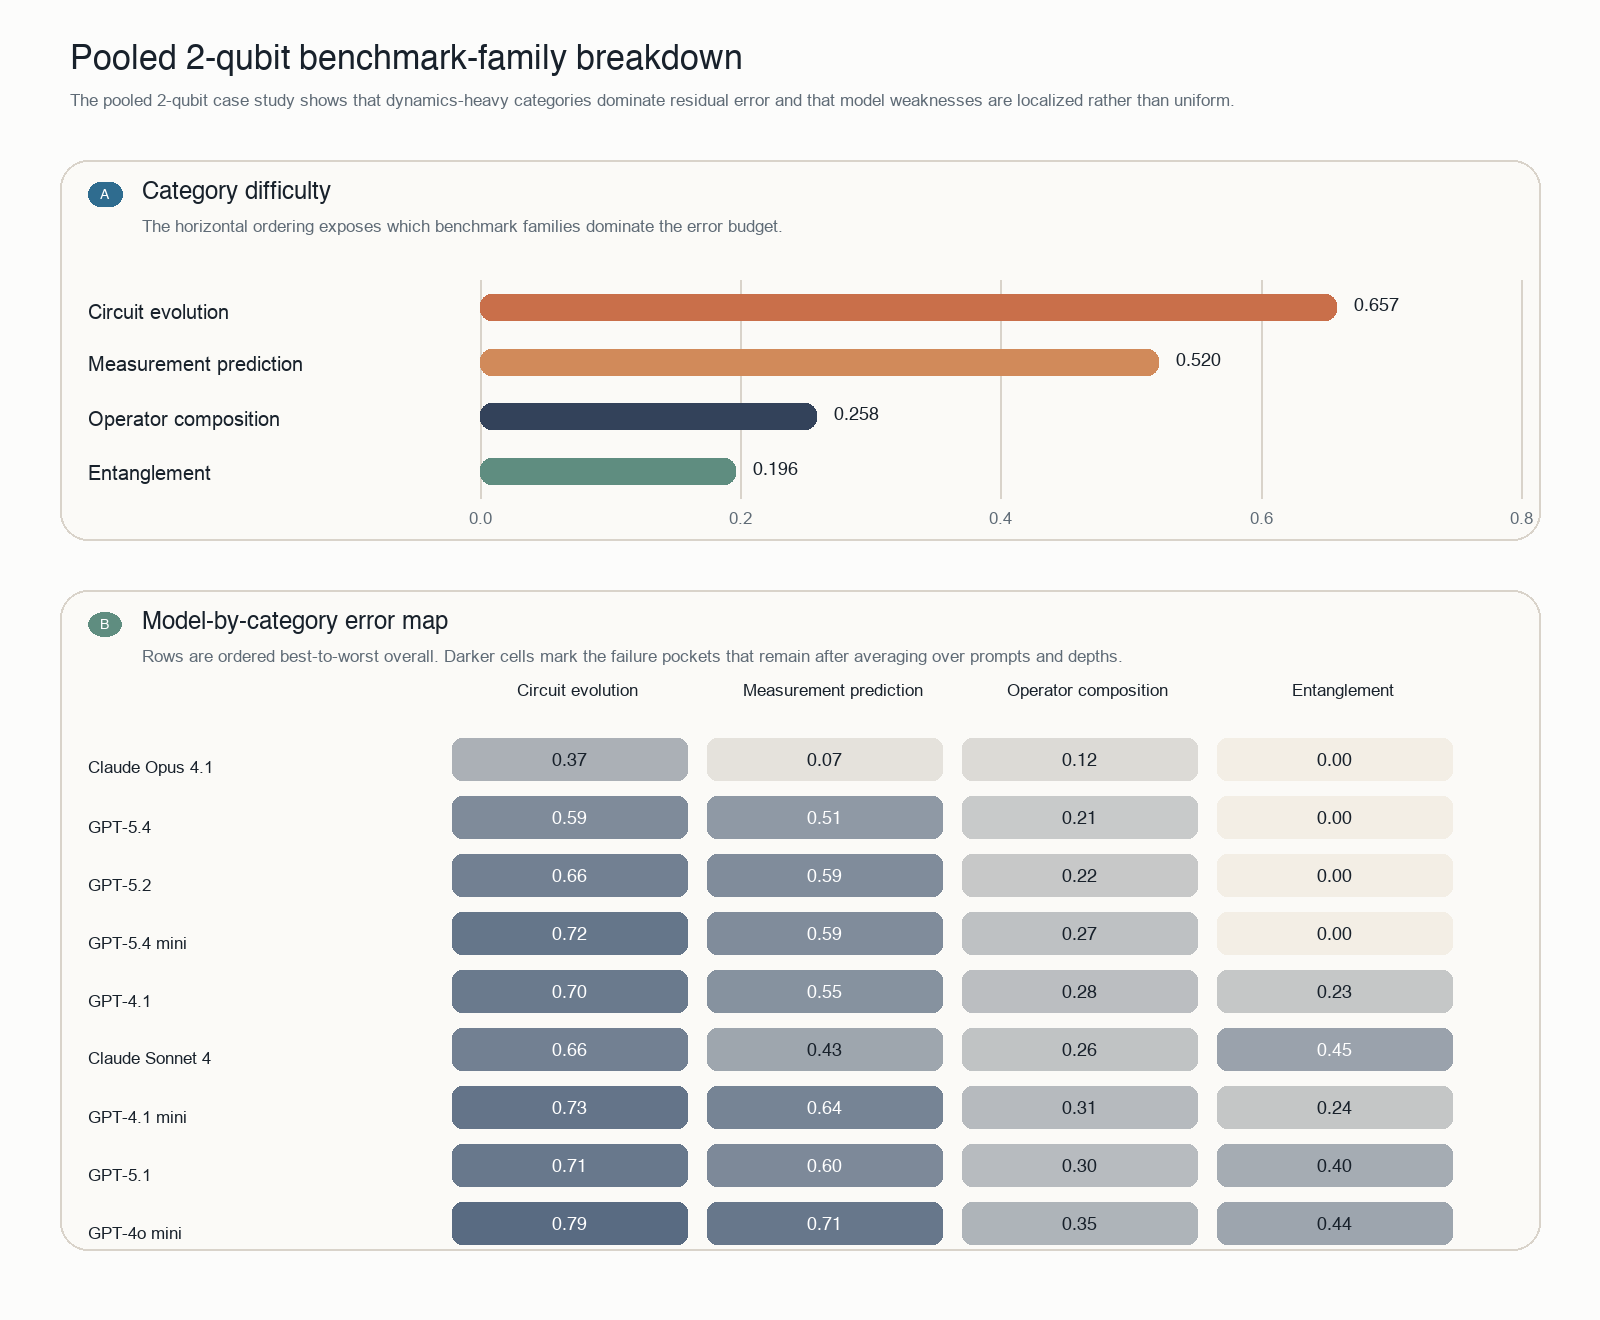
\includegraphics[width=\linewidth]{figures/combined_quantum_breakdown.png}
\caption{Benchmark-family breakdown in the pooled case study. Top: overall category difficulty. Bottom: model-by-category heatmap showing where each model fails most strongly.}
\label{fig:breakdown}
\end{figure}

\subsection{4-Qubit Stress Test}
The matched 4-qubit stress test shows that benchmark difficulty rises substantially once the state space is enlarged. Across the same GPT and Claude model sets, overall mean normalized error increases from 0.408 on the 2-qubit benchmark to 0.533 on the 4-qubit benchmark, a delta of $+0.125$. If we restrict attention to the three categories that actually scale from 2 to 4 qubits, the increase is larger: GPT models rise by $+0.166$ on average, and Claude models rise by $+0.192$.

The degradation is concentrated in the same places that were already hardest in the main benchmark. In the pooled 2q$\rightarrow$4q comparison, circuit evolution increases by $+0.185$ and measurement prediction by $+0.188$. Entanglement classification also worsens by $+0.142$, while operator composition changes by $-0.013$ because it is intentionally held fixed as a one-qubit control task.

\begin{figure}[tb]
\centering
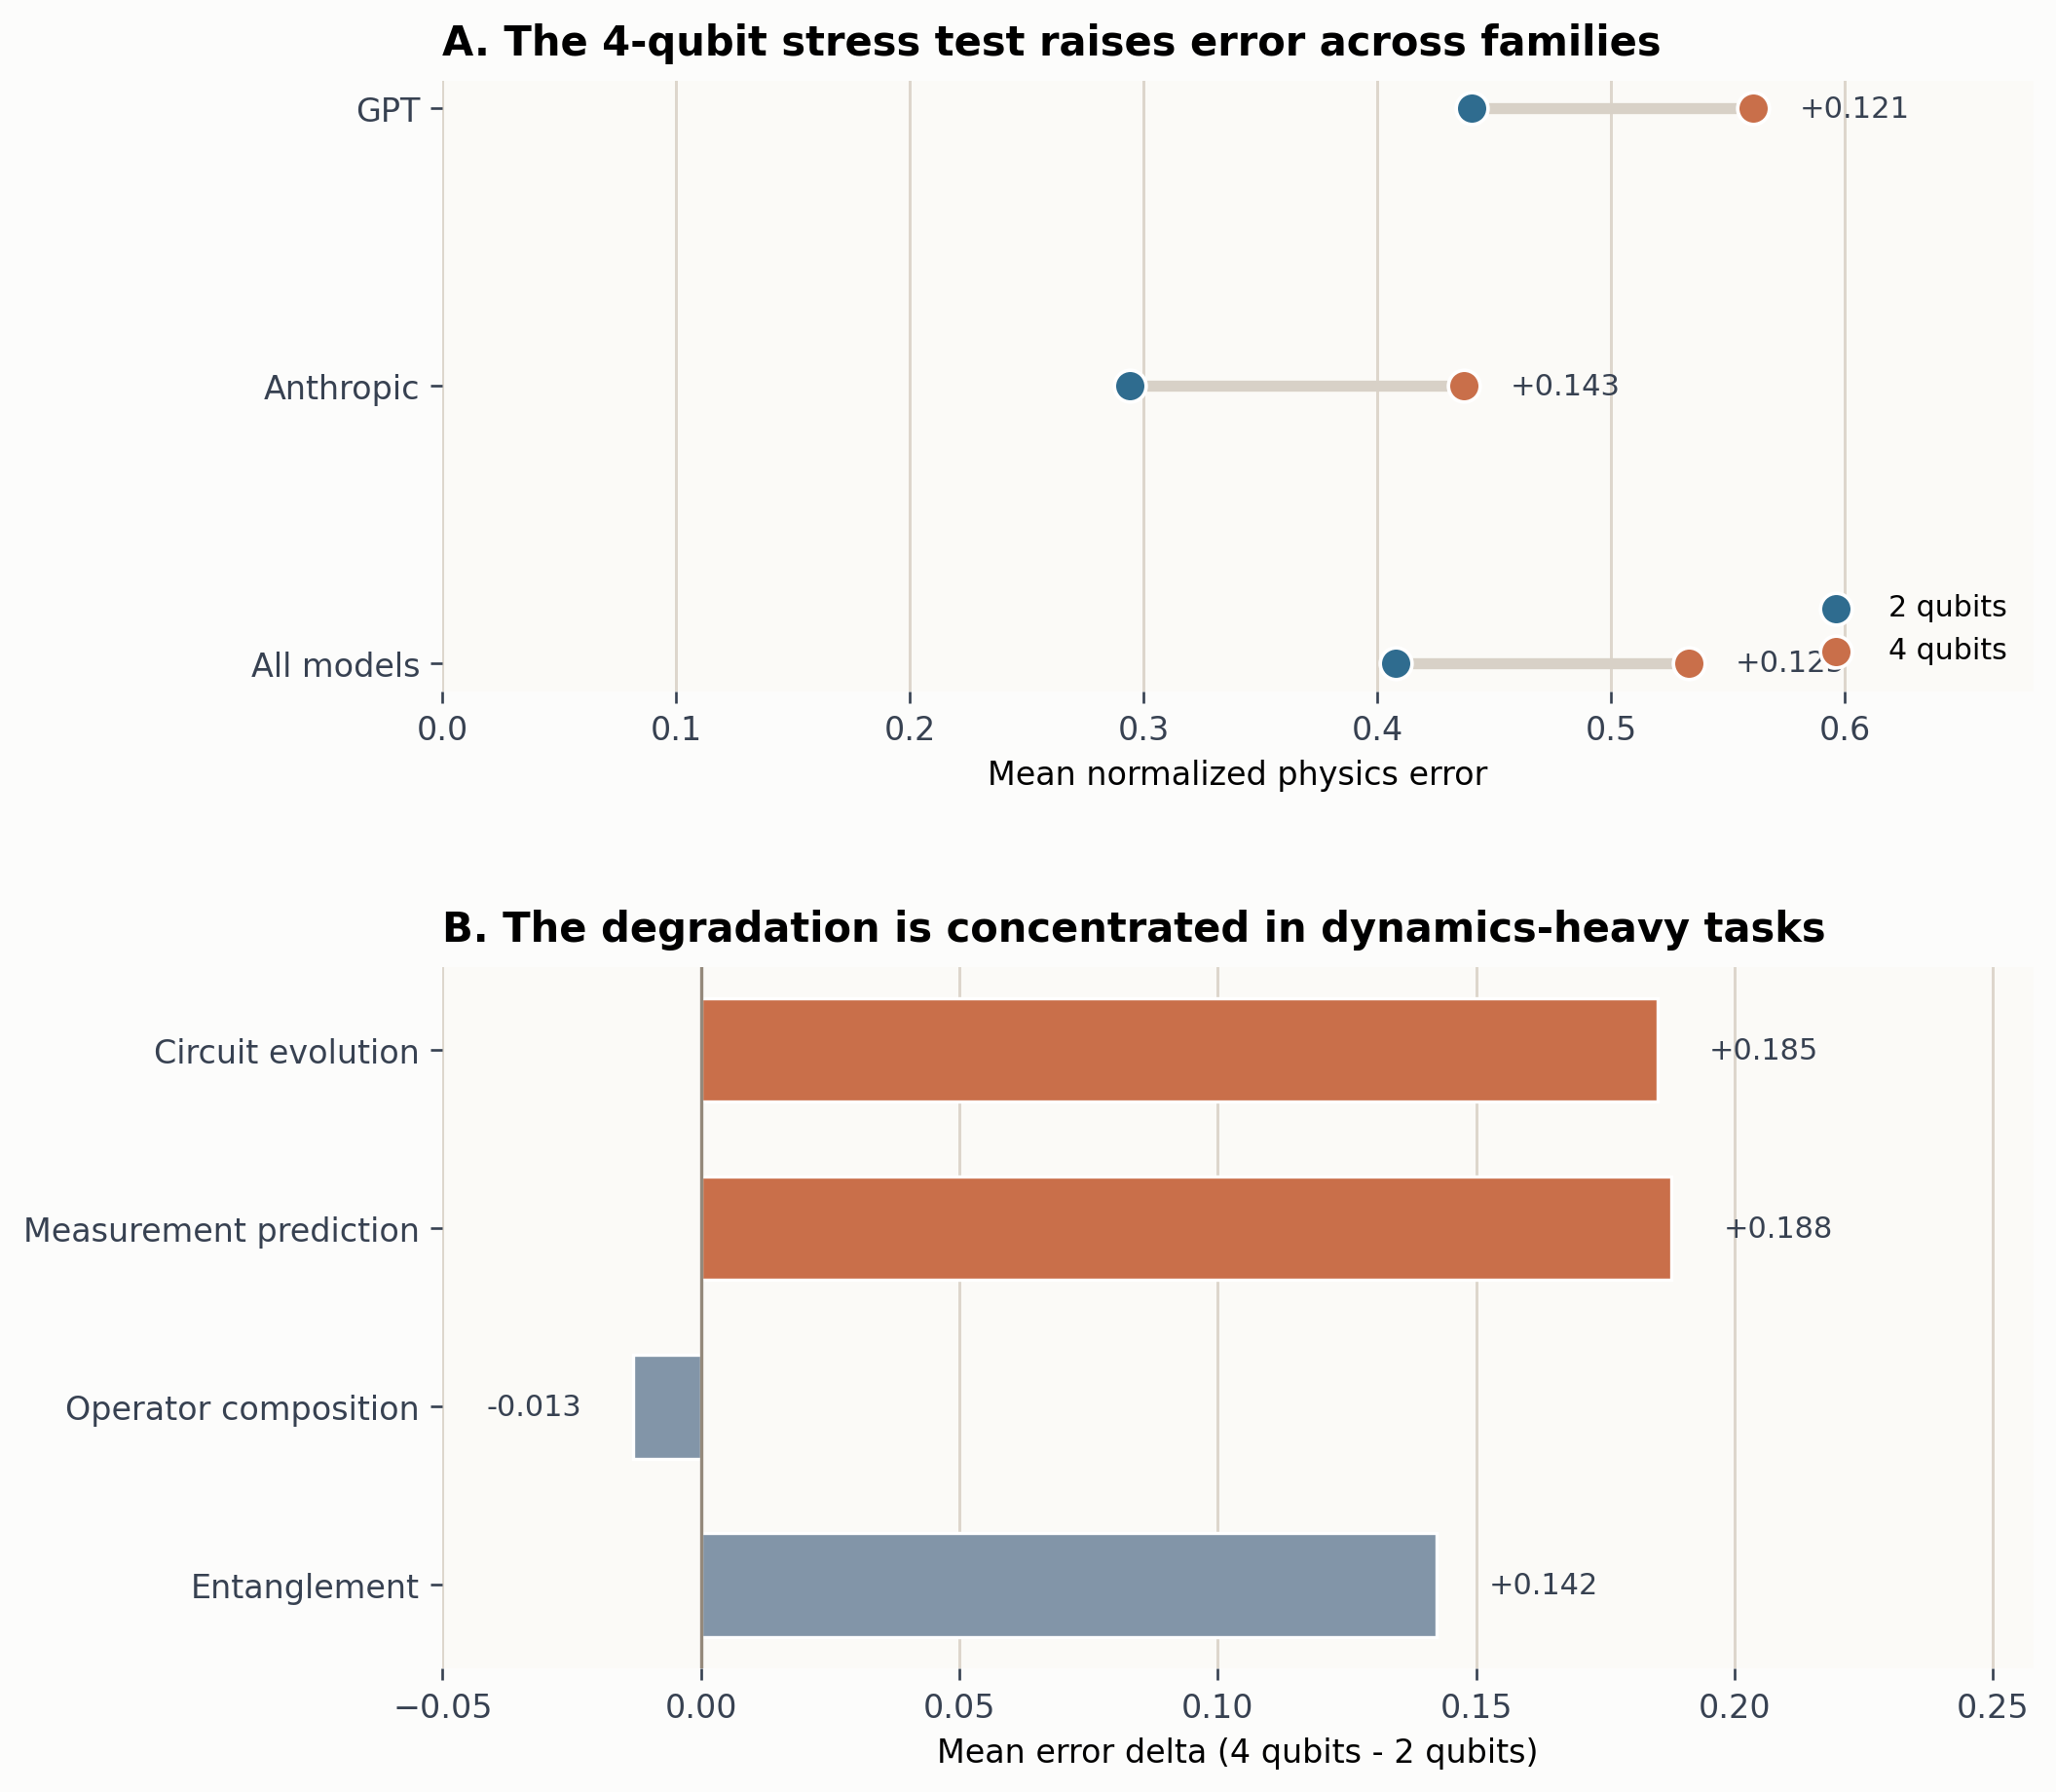
\includegraphics[width=\linewidth]{figures/qubit_stress_test.png}
\caption{Matched 2-qubit versus 4-qubit stress test. Top: both GPT and Claude families get worse when the benchmark is rerun at 4 qubits. Bottom: the largest degradations occur in circuit evolution and measurement prediction, while the unchanged operator-composition control slice remains nearly flat.}
\label{fig:qubit-stress}
\end{figure}

\begin{figure}[tb]
\centering

\includegraphics[width=\linewidth]{figures/combined_4qubit_breakdown.png}
\caption{Benchmark-family breakdown in the pooled 4-qubit case study. Top: overall category difficulty at 4 qubits. Bottom: model-by-category heatmap showing where 4-qubit failures remain concentrated.}
\label{fig:breakdown-4q}
\end{figure}

\subsection{Complexity Scaling to 8 Qubits}
The completed Anthropic 2q$\rightarrow$4q$\rightarrow$8q ladder shows that the state-space trend continues beyond the pooled 4-qubit stress test. Mean normalized error rises monotonically from 0.294 at 2 qubits to 0.437 at 4 qubits and 0.542 at 8 qubits, for a total 2q$\rightarrow$8q increase of $+0.248$. The distribution also becomes harsher as qubit count grows: the exact-correct rate falls from 59.0\% at 2 qubits to 44.9\% at 4 qubits and 35.2\% at 8 qubits, while the full-error rate rises from 20.7\% to 34.6\% to 48.3\%.

The strongest complexity signal remains concentrated in exact quantum dynamics. Across the Anthropic ladder, circuit evolution rises from 0.512 to 0.573 to 0.900, and measurement prediction rises from 0.250 to 0.514 to 0.760. By contrast, operator composition stays almost perfectly flat at 0.187, 0.182, and 0.188. This is the key control result: the 8-qubit degradation is not just a generic penalty for longer prompts or longer outputs. It is primarily a failure of exact amplitude and probability tracking as the Hilbert space grows.

The same pattern holds within individual Anthropic models. Claude Opus 4.1 rises from 0.138 at 2 qubits to 0.298 at 4 qubits and 0.445 at 8 qubits. Claude Sonnet 4 rises from 0.450 to 0.576 to 0.640. Stronger capability therefore improves the baseline, but it does not remove the complexity trend. The one notable exception is entanglement classification, which is noisier as a complexity probe: it rises from 0.227 to 0.479 and then drops to 0.320 at 8 qubits. We therefore treat the cleanest complexity evidence as coming from circuit evolution, measurement prediction, and the flat operator-composition control.

\begin{figure}[tb]
\centering
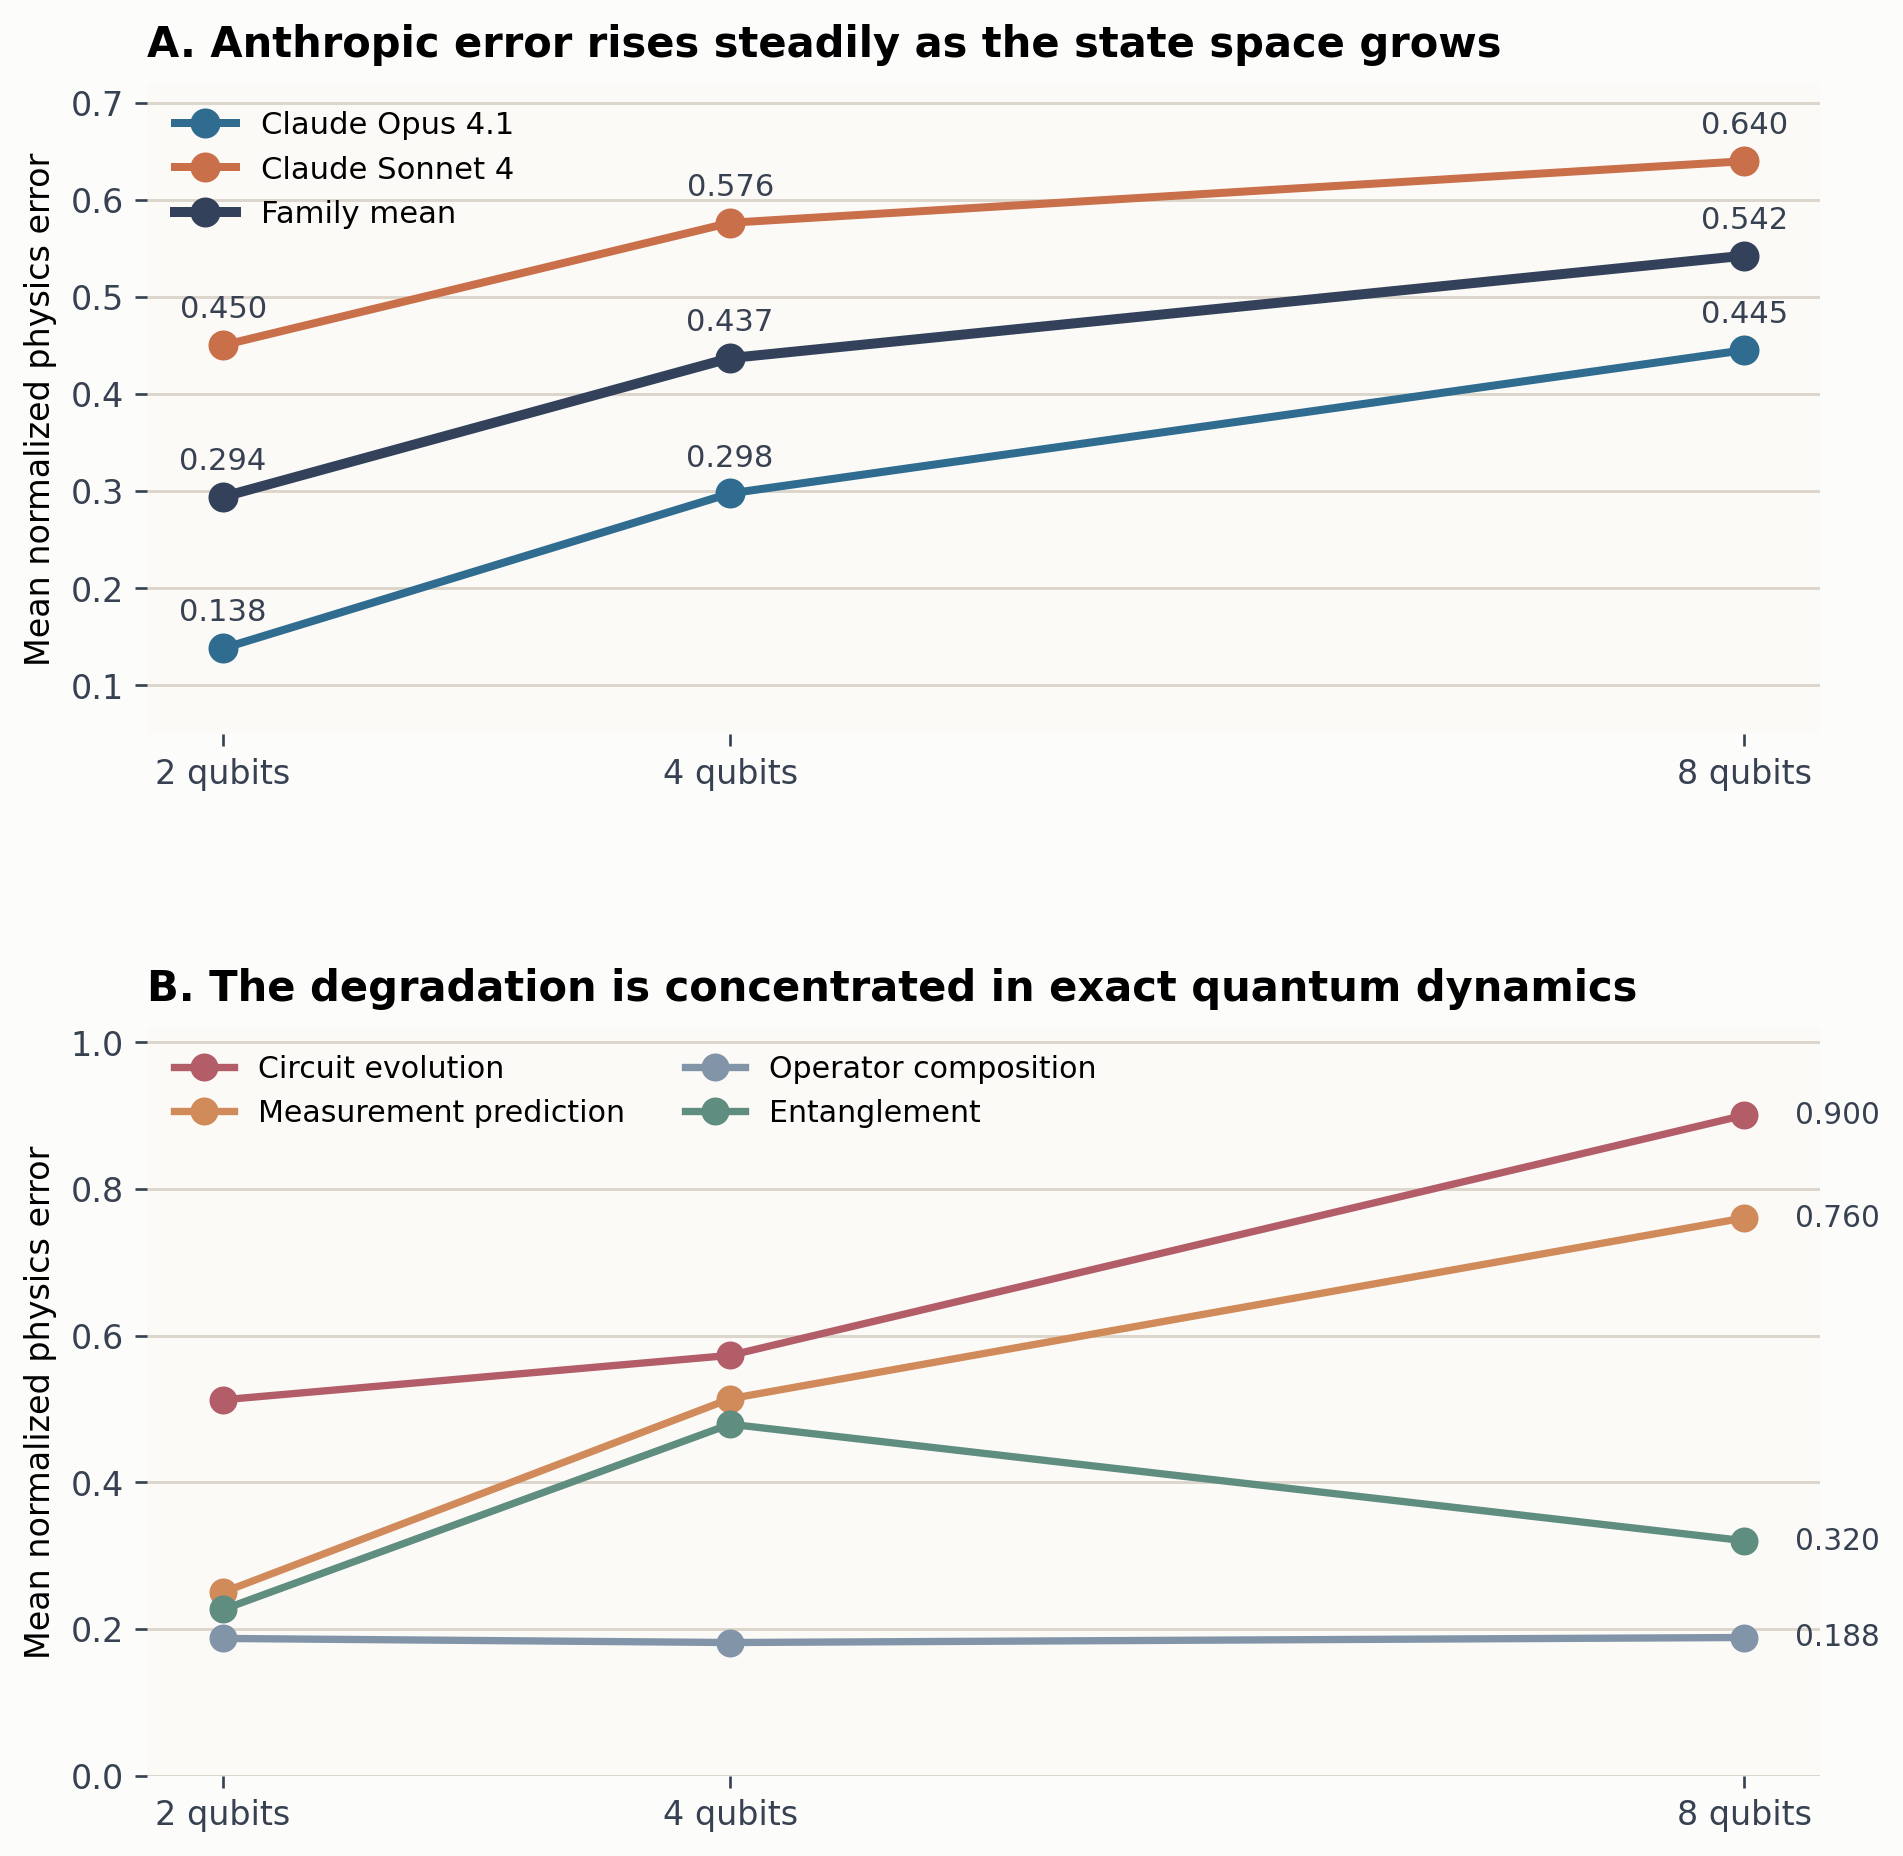
\includegraphics[width=\linewidth]{figures/anthropic_complexity_scaling.png}
\caption{Completed Anthropic 2q$\rightarrow$4q$\rightarrow$8q complexity ladder. Top: both Claude models and the Anthropic family mean degrade monotonically as qubit count rises. Bottom: the sharpest growth is in circuit evolution and measurement prediction, while the fixed operator-composition control slice remains nearly unchanged.}
\label{fig:complexity-scaling}
\end{figure}

\begin{figure}[tb]
\centering
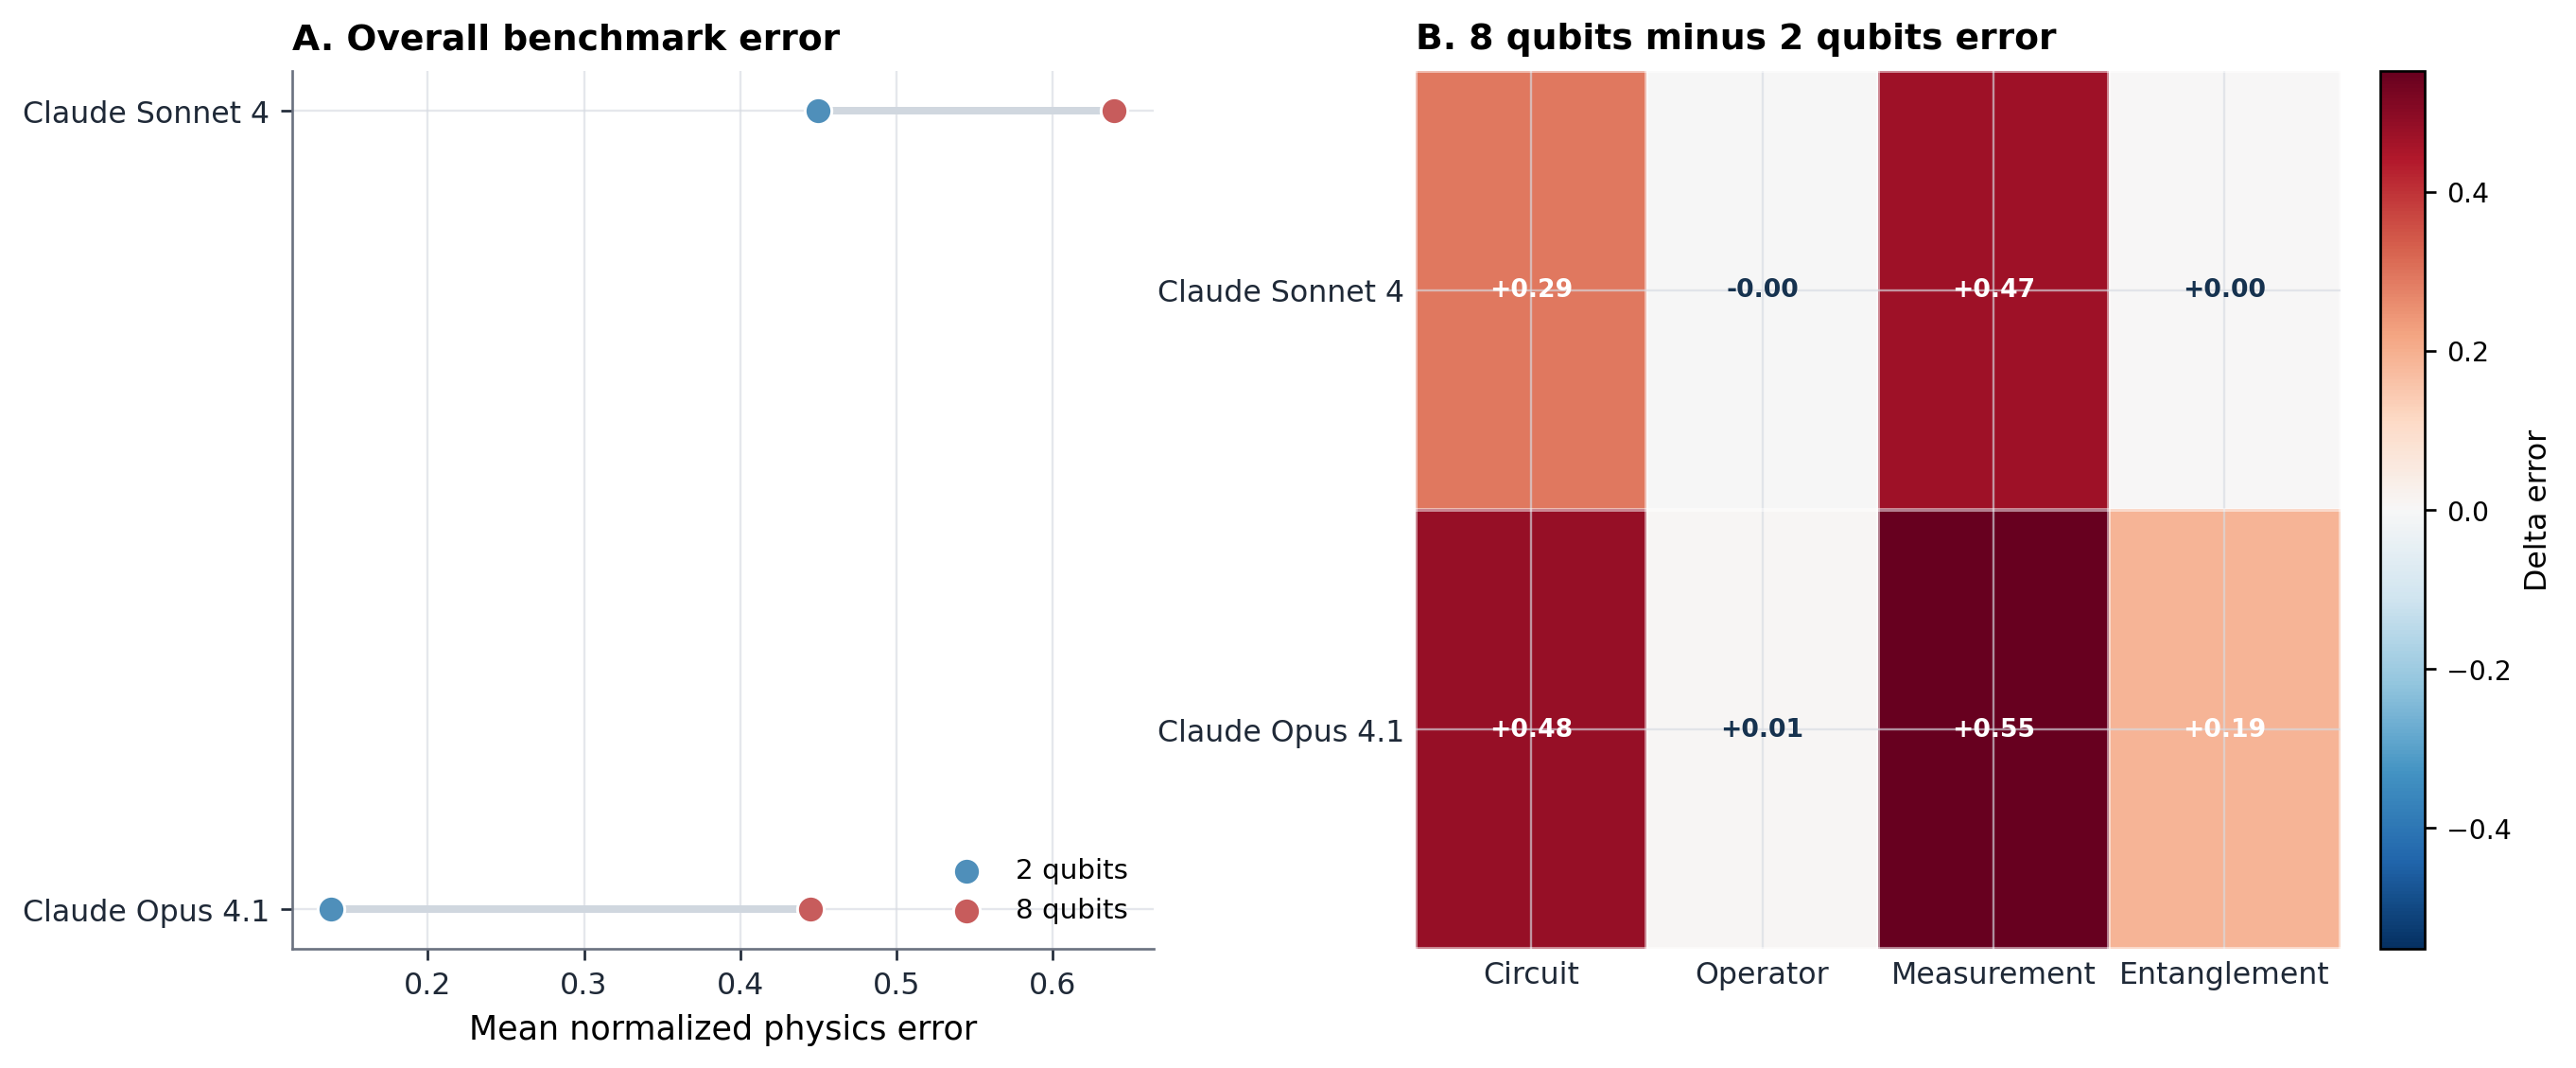
\includegraphics[width=\linewidth]{figures/anthropic_2q_vs_8q.png}
\caption{Anthropic 2-qubit versus 8-qubit stress comparison in the same visual format as the smaller stress-test figures. Top: both Claude models worsen substantially by 8 qubits. Bottom: the largest 2q$\rightarrow$8q increases remain circuit evolution and measurement prediction, while operator composition stays flat as a control.}
\label{fig:qubit-stress-8q}
\end{figure}

\begin{figure}[tb]
\centering
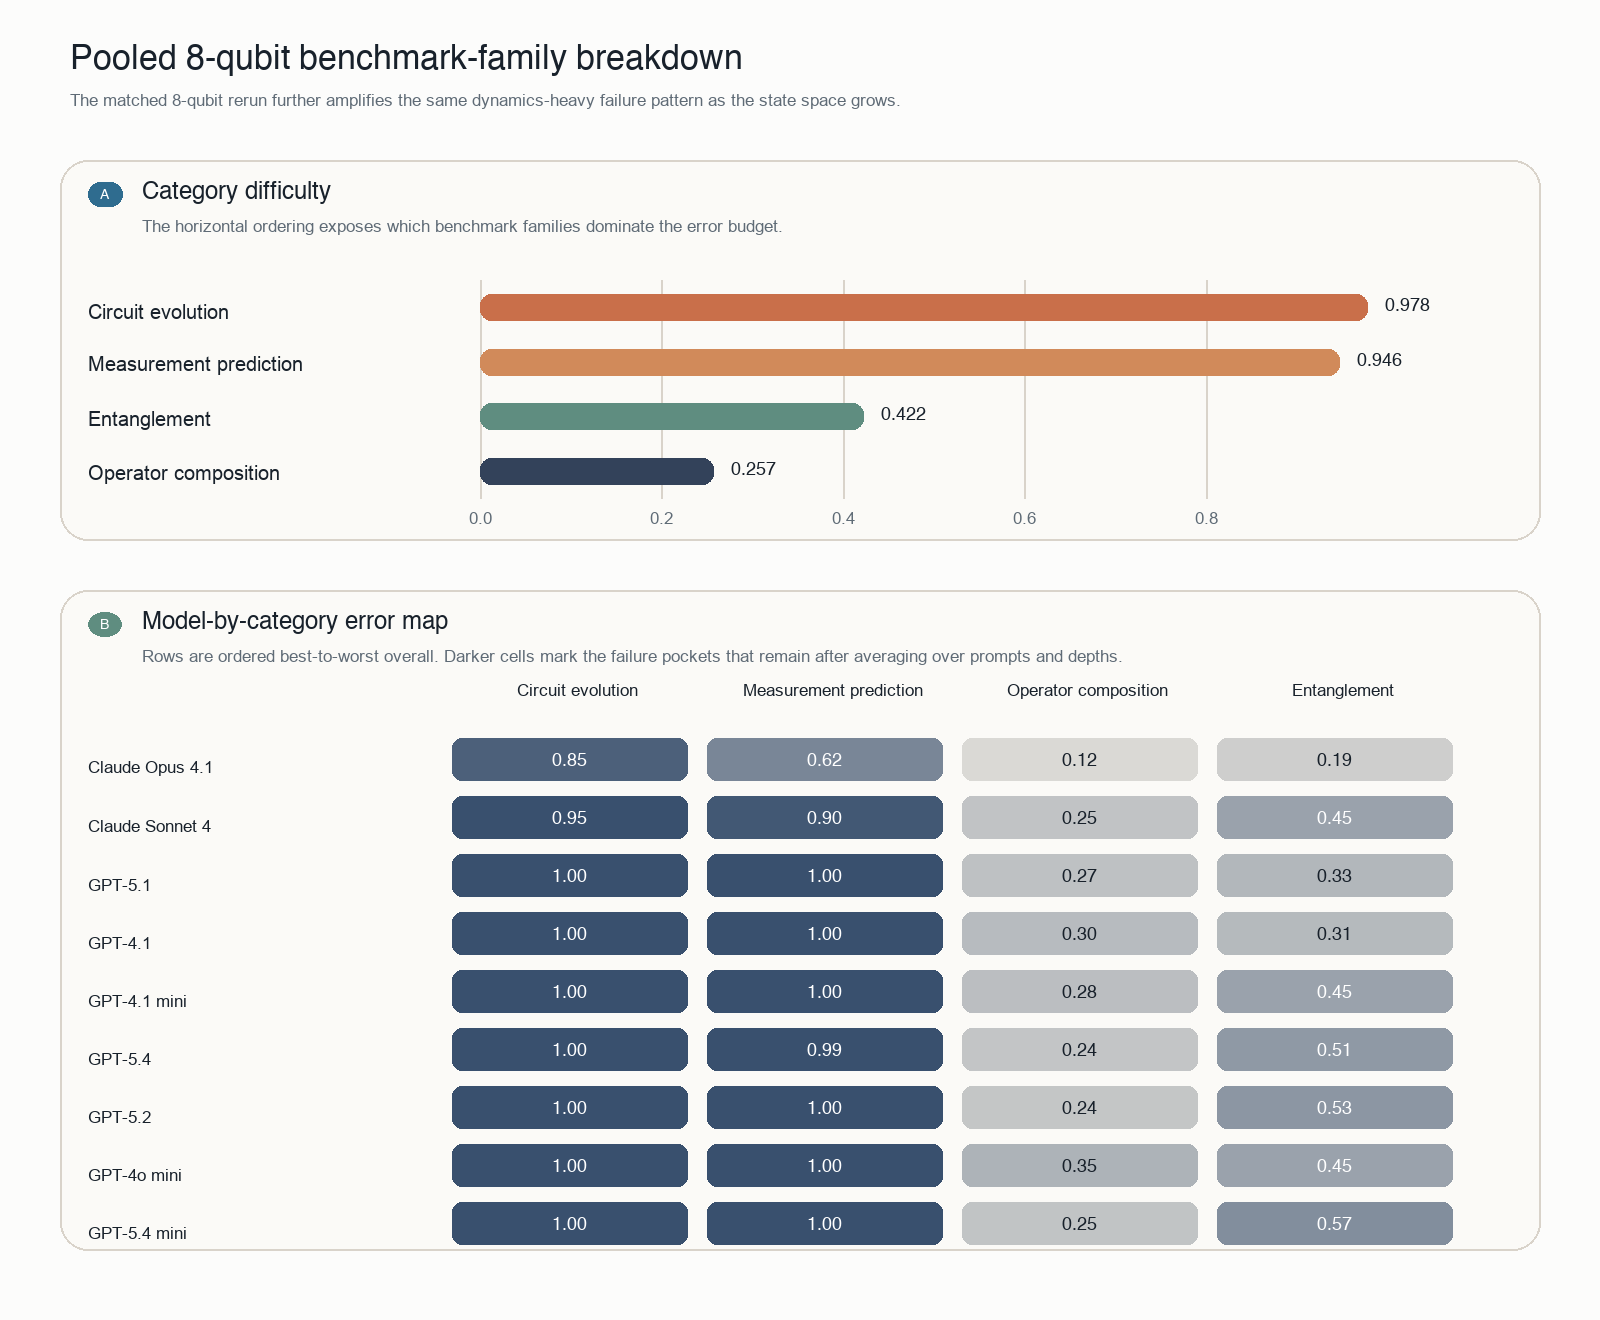
\includegraphics[width=\linewidth]{figures/combined_8qubit_breakdown.png}
\caption{Benchmark-family breakdown in the completed 8-qubit Anthropic rerun. Top: category difficulty at 8 qubits. Bottom: model-by-category heatmap showing that both Claude models remain most vulnerable on circuit evolution and measurement prediction.}
\label{fig:breakdown-8q}
\end{figure}

The completed GPT 2q$\rightarrow$4q$\rightarrow$8q ladder now shows the same state-space trend at larger scale. Across 5{,}374 usable GPT 8-qubit responses, family mean error rises from 0.440 at 2 qubits to 0.561 at 4 qubits and 0.682 at 8 qubits. The distribution becomes harsher in the same way as the Anthropic ladder: exact-correct rate is only 18.2\% at 8 qubits, while the full-error rate rises to 61.3\%.

The GPT category pattern closely matches the completed Anthropic result. Circuit evolution reaches 1.000 mean error at 8 qubits, measurement prediction reaches 0.999, entanglement classification reaches 0.451, and operator composition remains much lower at 0.277. This again supports the same interpretation: the dominant complexity effect is not a generic formatting penalty, but a collapse in exact quantum-dynamics tracking as the Hilbert space grows.

The model-level GPT ranking also stabilizes in the completed 8-qubit file. \texttt{gpt-5.1} is the strongest GPT slice at 0.649 mean error, closely followed by \texttt{gpt-4.1} at 0.654. \texttt{gpt-5.4} reaches 0.686 over 766 usable rows, \texttt{gpt-5.2} reaches 0.691, \texttt{gpt-4o-mini} reaches 0.702, and \texttt{gpt-5.4-mini} reaches 0.706. Even the strongest GPT slices therefore remain far worse at 8 qubits than on the smaller-qubit benchmarks, and they remain qualitatively aligned with the Anthropic story.

\begin{figure}[tb]
\centering
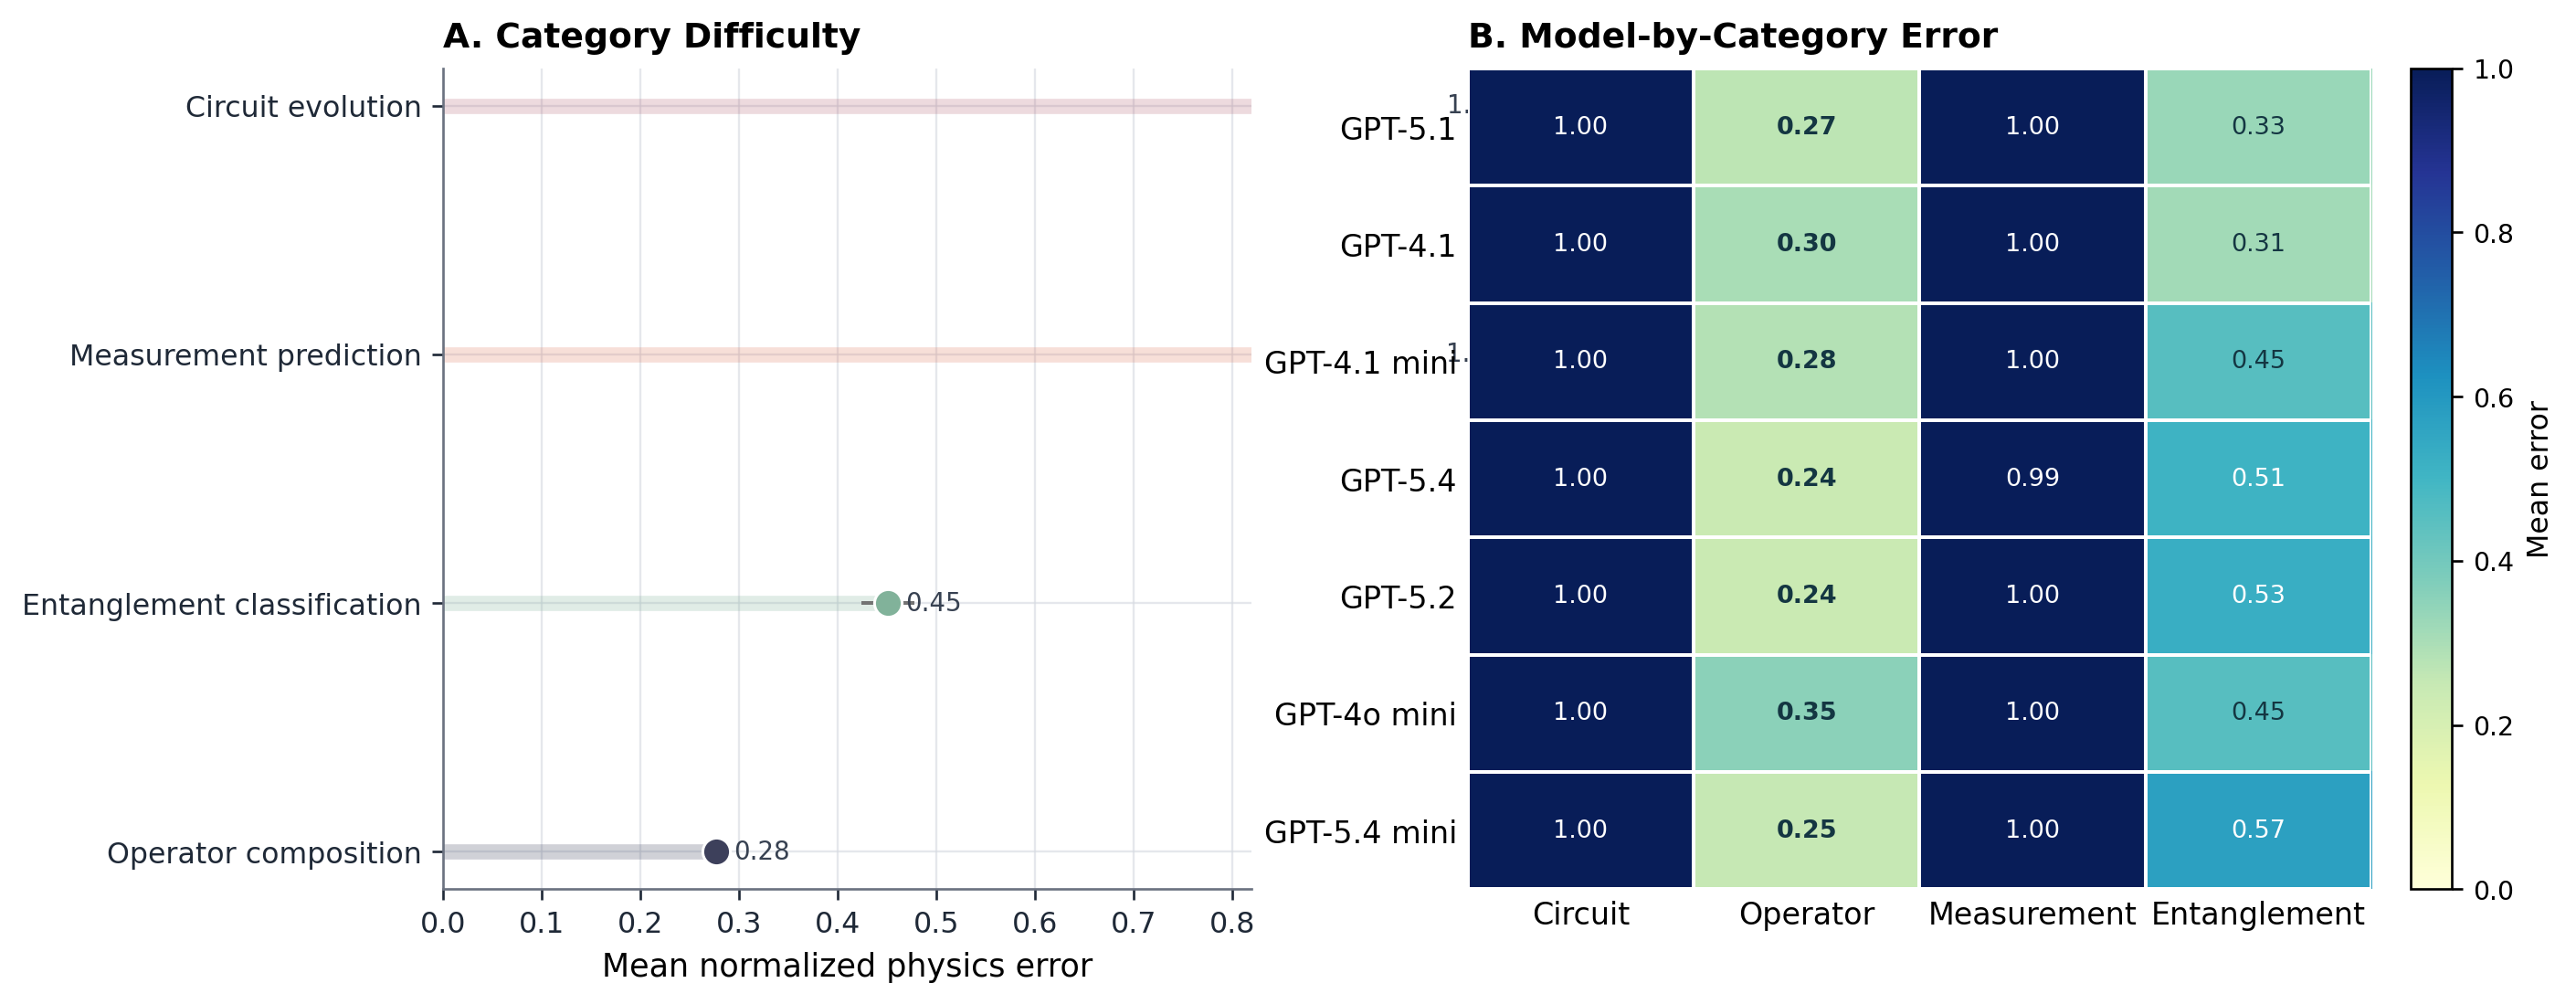
\includegraphics[width=\linewidth]{figures/gpt_8qubit_breakdown.png}
\caption{Completed GPT 8-qubit run. Top: category difficulty on the 5{,}374 usable-response file. Bottom: model-by-category heatmap. The same pattern visible in the Anthropic ladder persists here: circuit evolution and measurement prediction saturate, while operator composition remains substantially lower.}
\label{fig:gpt-8q-checkpoint}
\end{figure}

\begin{figure}[tb]
\centering
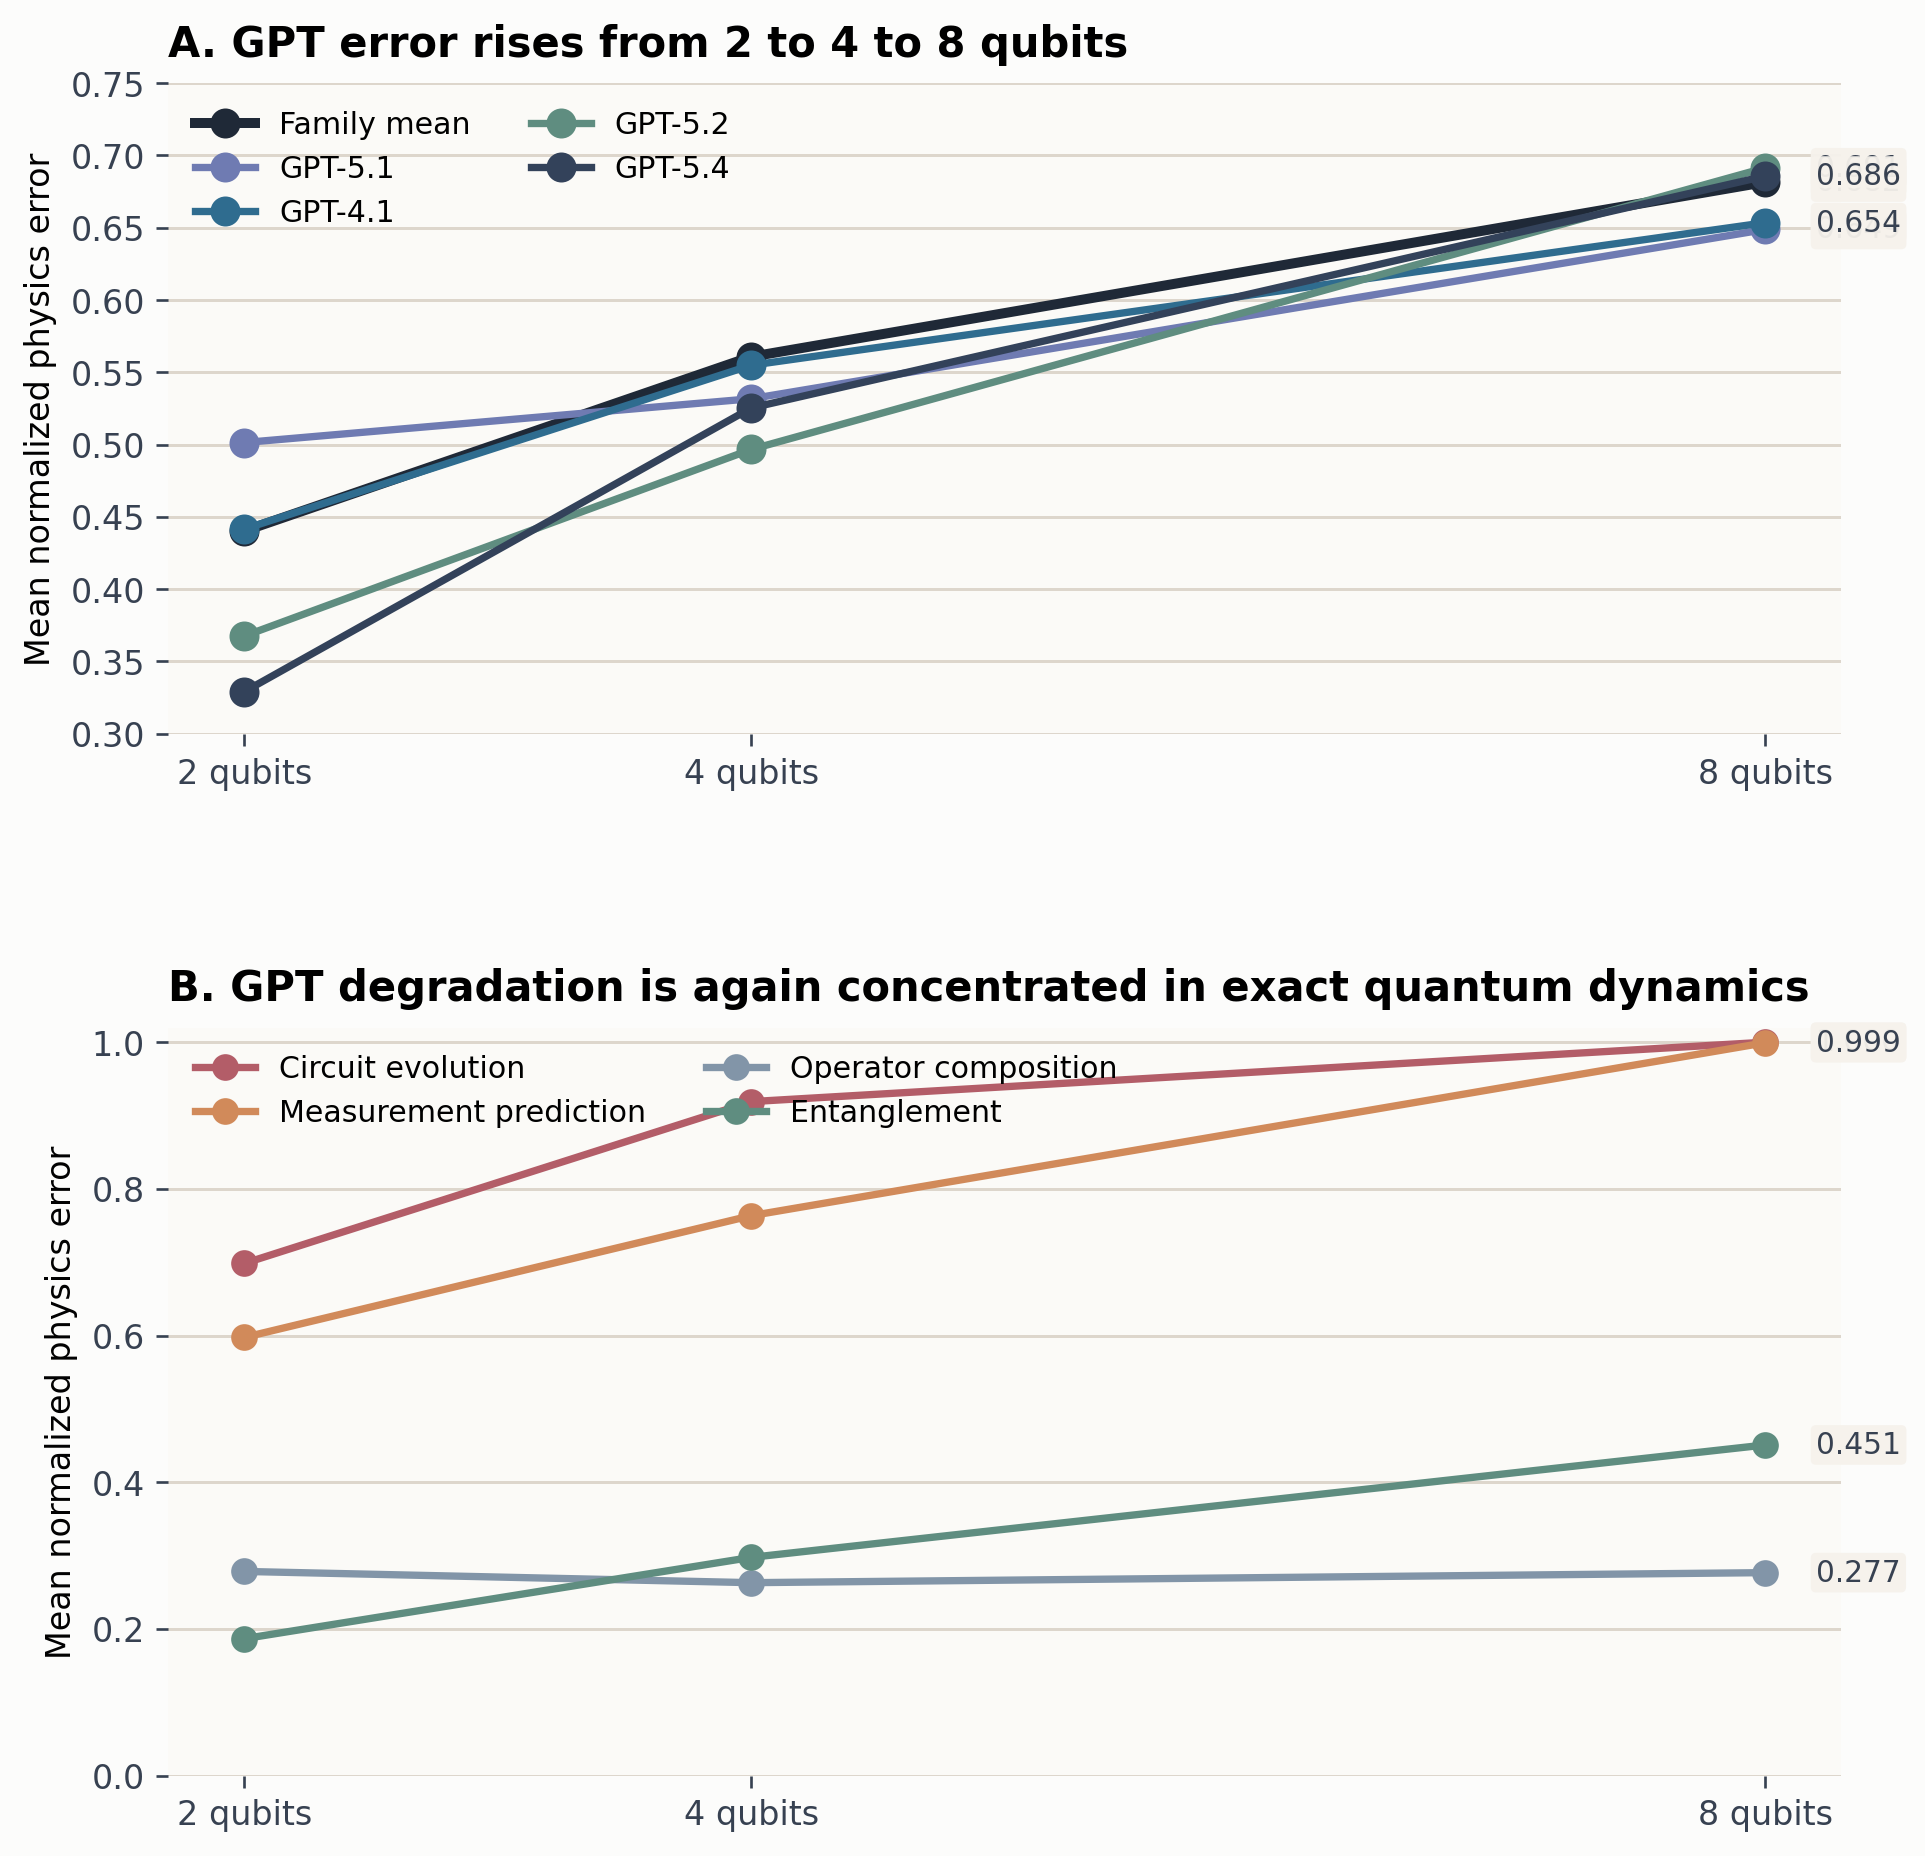
\includegraphics[width=\linewidth]{figures/gpt_complexity_scaling.png}
\caption{Completed GPT 2q$\rightarrow$4q$\rightarrow$8q complexity ladder. Top: the GPT family mean and representative stronger GPT slices all worsen as qubit count rises. Bottom: the sharpest increase remains in circuit evolution and measurement prediction, while operator composition stays comparatively flat.}
\label{fig:gpt-complexity-scaling}
\end{figure}

\subsection{Ablations}
The repair ablation adds a more operational view of the benchmark. Repeated attempts help substantially, but verifier-guided retry helps more than blind self-retry. Solved fraction rises from 0.422 in the one-shot condition to 0.609 under self-retry and 0.688 under verifier feedback. The time-budget curves flatten quickly: in the verifier-feedback run, pass@30s, pass@60s, pass@120s, and pass@300s are all equal to 0.688.

\begin{figure}[tb]
\centering
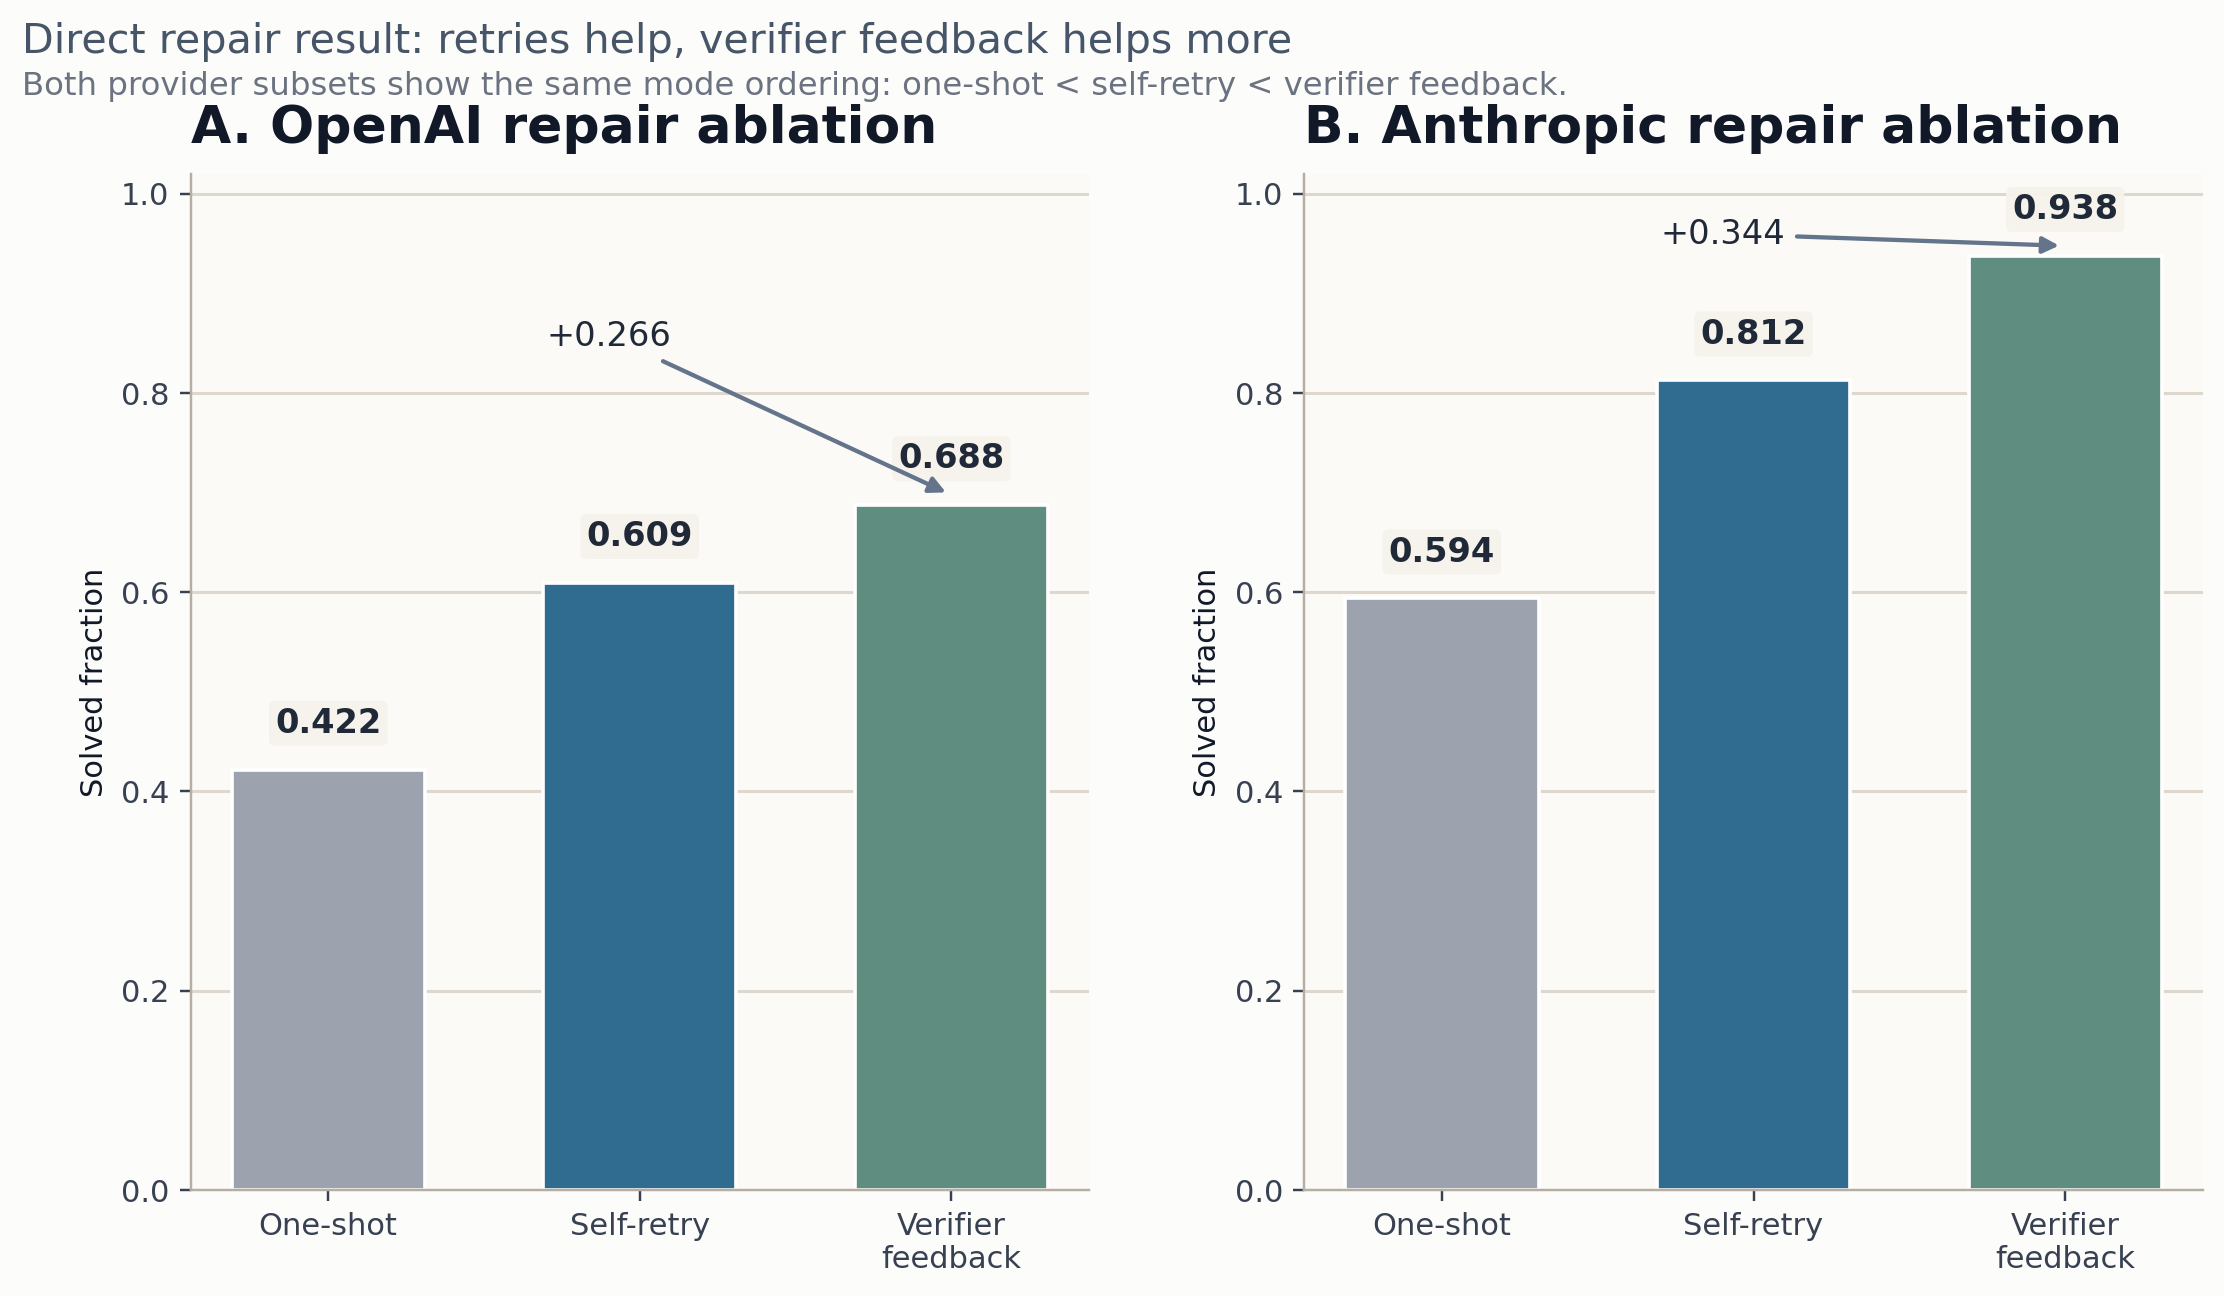
\includegraphics[width=\linewidth]{figures/feedback_ablation_summary.png}
\caption{Direct comparison of repair modes. In both the OpenAI and Anthropic subsets, solved fraction rises monotonically from one-shot to self-retry to verifier feedback. This makes the core ablation result visible at a glance rather than only through the table.}
\label{fig:feedback-summary}
\end{figure}

\begin{figure}[tb]
\centering
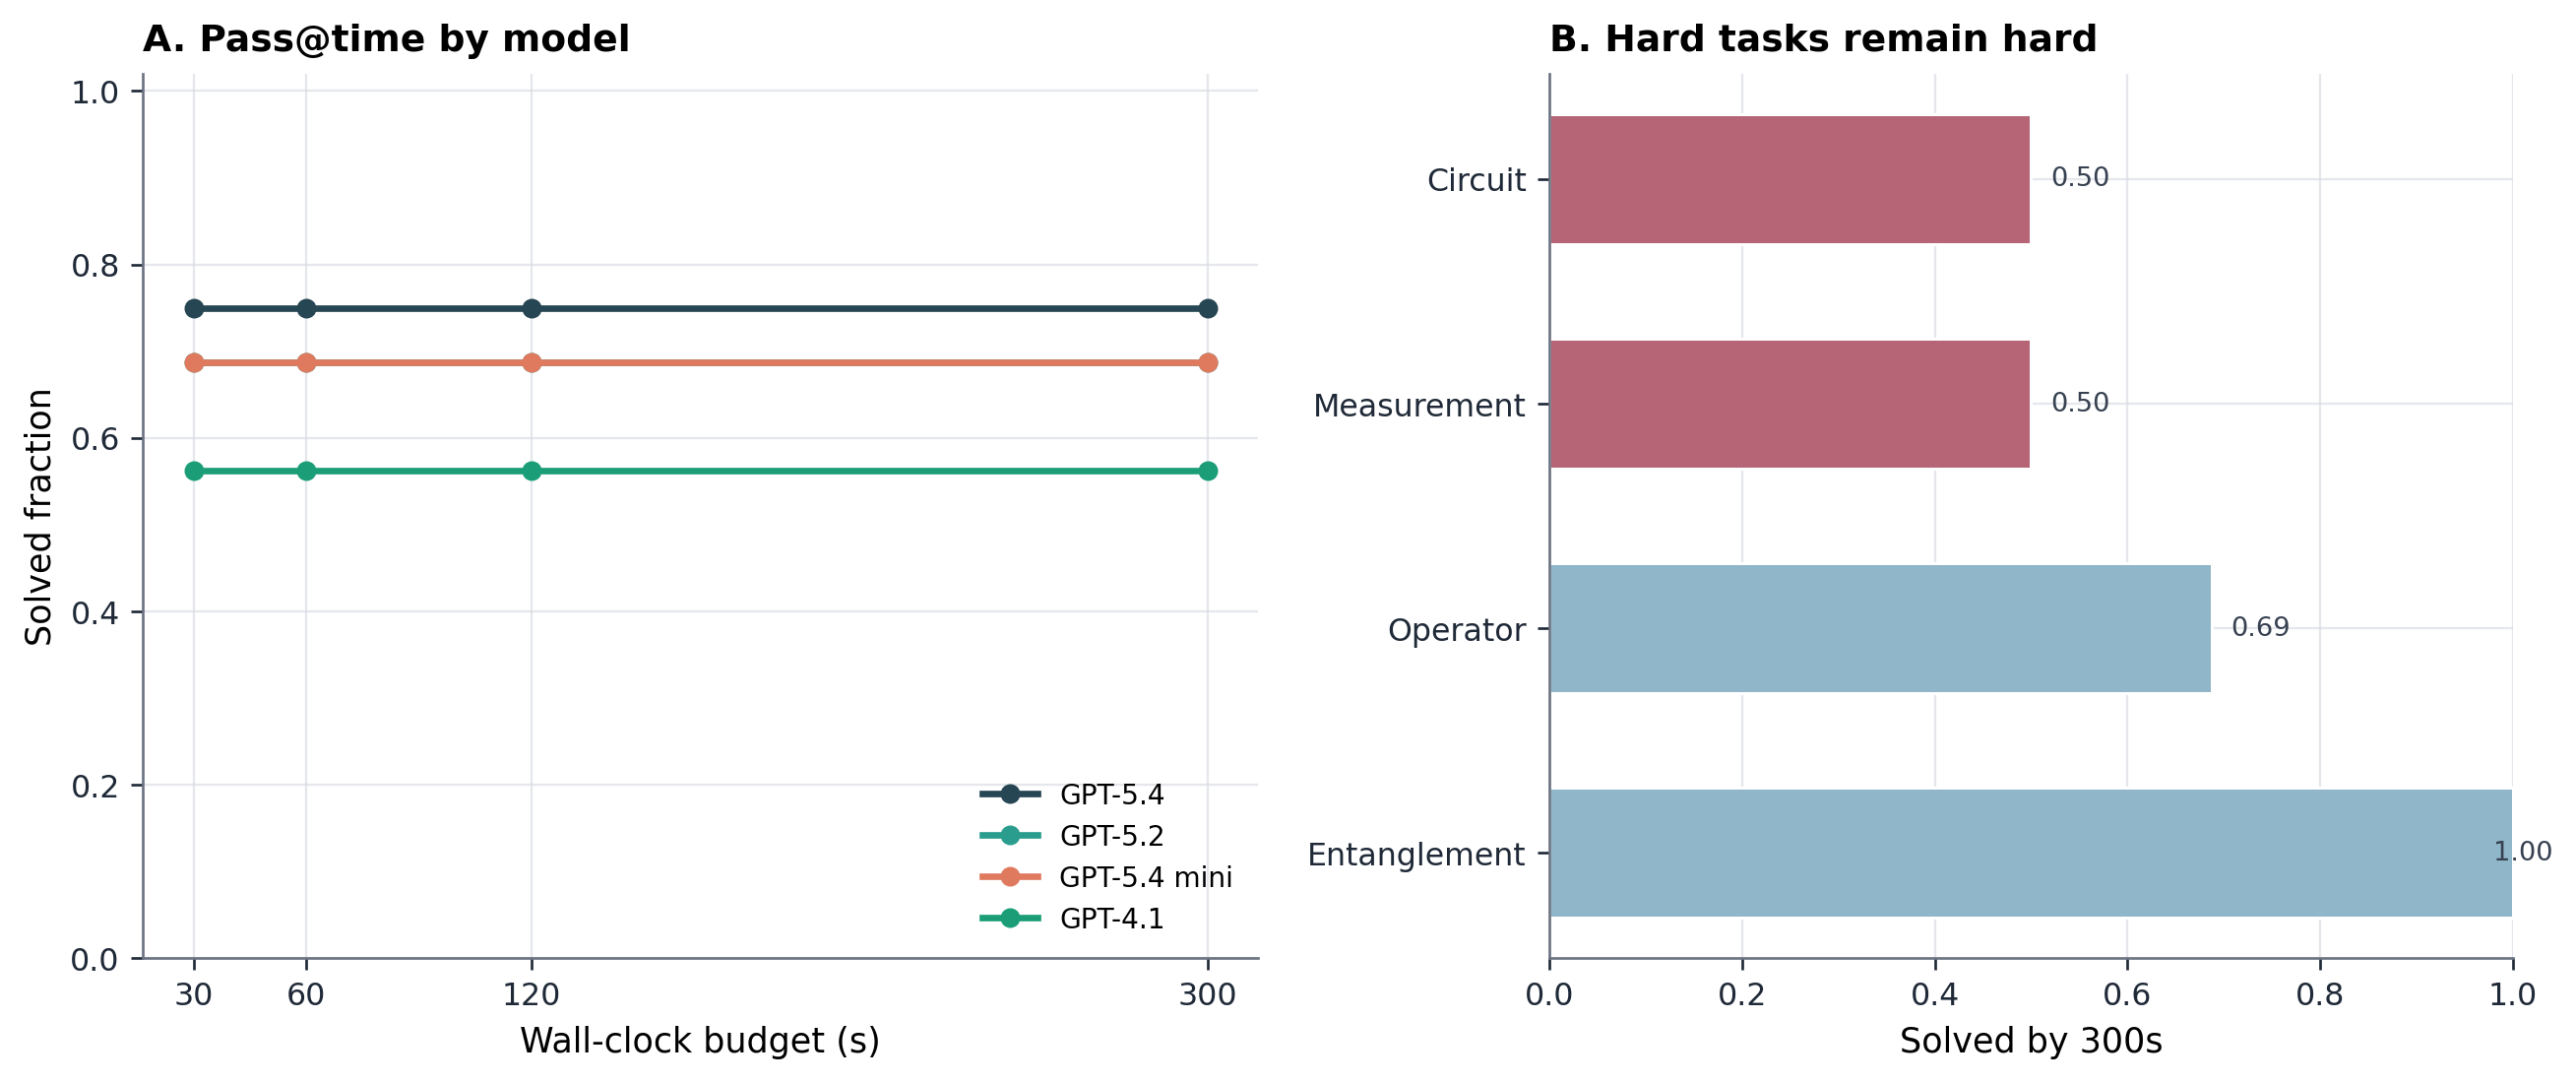
\includegraphics[width=\linewidth]{figures/timebudget_strong_models_progress.png}
\caption{Verifier-feedback time-budget run on the strong-model subset. Left: solved fraction by wall-clock budget for each model. Right: solved fraction by category under the full 300-second budget.}
\label{fig:timebudget}
\end{figure}

We observe the same qualitative pattern on the Claude subset once output extraction is made robust to mixed prose and code-block responses. On a matched 32-task Anthropic subset using Claude Sonnet 4 and Claude Opus 4.1, solve rate rises from 0.594 in the one-shot condition to 0.813 under self-retry and 0.938 under verifier feedback.

\section{Related Work}
QuantumPhysEval is most closely related to benchmark efforts that favor exact or programmatic scoring over free-form human judgment. In broad LLM evaluation, HELM, BIG-bench, and MMLU established the value of standardized cross-model measurement, but they are not designed to test exact physical consistency in scientific state-tracking tasks \citep{liang2023helm,srivastava2023beyond,hendrycks2021mmlu}. In code generation, HumanEval showed how executable or exact ground truth can make evaluation sharper and more reproducible \citep{chen2021evaluating}. In safety and domain-specific evaluation, benchmarks such as Asleep at the Keyboard and CyberSecEval demonstrated that narrow, operationally grounded suites can expose failure modes that broad capability tests miss \citep{pearce2022asleep,bhatt2023purple}. QuantumPhysEval follows that benchmark-first tradition, but targets exact quantum-mechanical validity: normalization, unitarity, state evolution, measurement probabilities, and entanglement status.

This paper also sits near recent work on scientific and mathematical reasoning in language models. Existing broad science or math benchmarks can reveal whether a model reaches the right answer, but they usually do not distinguish between a response that is merely wrong and one that is physically inconsistent while still plausible. Our focus is narrower: we aim to measure whether language models preserve exact quantum structure under controlled small-system conditions, and how that reliability changes with model family, prompted depth, verifier feedback, and state-space size.

\section{Discussion}
The case study supports five practical conclusions. First, quantum hallucination is measurable in a fully automated setting. Second, model capability matters more than prompted depth in the present setup. Third, some failures are recoverable under iterative interaction, but the mechanism matters: verifier-guided retry helps more than blind self-retry. Fourth, the benchmark identifies a concrete residual weakness in exact quantum state and probability evolution. Fifth, the matched 4-qubit stress test and completed Anthropic 8-qubit ladder show that these failures do not remain confined to the easiest possible small systems: error continues to rise as the state space grows, and the growth remains concentrated in the same dynamics-heavy categories.

\section{Limitations}
QuantumPhysEval is intentionally narrow. It uses controlled small-system settings to enable exact scoring, but that also limits ecological breadth. Even with the added 4-qubit stress test and the completed Anthropic and GPT 8-qubit ladders, the benchmark remains far from realistic chemistry, control, or error-correction workloads. The model-size variable is a manually assigned proxy rather than a verified parameter count, and the pooled fit mixes families and release generations. The larger-qubit stress tests do not upscale operator composition, since returning exact 16$\times$16 or 64$\times$64 matrices would mostly measure formatting burden rather than useful reasoning. The completed GPT 8-qubit file still contains two residual API failures, but at 5{,}374 usable responses the qualitative pattern is stable and matches the Anthropic ladder.

\section{Conclusion}
QuantumPhysEval provides a benchmark for measuring quantum hallucinations as physics-grounded error on elementary quantum tasks. In a pooled 2-qubit case study over OpenAI GPT and Anthropic Claude models, benchmark error decreases strongly with model capability, while prompted reasoning depth shows no robust independent effect. A matched 4-qubit stress test shows that performance worsens materially once the state space expands, especially on circuit evolution and measurement prediction. A completed Anthropic 8-qubit ladder shows that this is a genuine complexity trend rather than a one-step artifact: error continues to rise, exact-correct rate falls, and full-error failures become more common as the Hilbert space grows. These results suggest that language models can produce plausible quantum answers, but exact physical reliability remains limited and should be measured explicitly rather than assumed.

\section*{References}
\begin{thebibliography}{9}

\bibitem[Bhatt et~al.(2023)]{bhatt2023purple}
Manish Bhatt, Sahana Chennabasappa, Cyrus Nikolaidis, Shengye Wan, Ivan Evtimov, Dominik Gabi, Daniel Song, Faizan Ahmad, Cornelius Aschermann, Lorenzo Fontana, Sasha Frolov, Ravi Prakash Giri, Dhaval Kapil, Yiannis Kozyrakis, David LeBlanc, James Milazzo, Aleksandar Straumann, Gabriel Synnaeve, Varun Vontimitta, Spencer Whitman, and Joshua Saxe.
\newblock Purple Llama CyberSecEval: A secure coding benchmark for language models.
\newblock arXiv preprint arXiv:2312.04724, 2023.

\bibitem[Chen et~al.(2021)]{chen2021evaluating}
Mark Chen, Jerry Tworek, Heewoo Jun, Qiming Yuan, Henrique Ponde de Oliveira Pinto, Jared Kaplan, Harri Edwards, Yuri Burda, Nicholas Joseph, Greg Brockman, Alex Ray, Raul Puri, Gretchen Krueger, Pamela Mishkin, Lilian Weng, Bob McGrew, Dario Amodei, and Ilya Sutskever.
\newblock Evaluating large language models trained on code.
\newblock arXiv preprint arXiv:2107.03374, 2021.

\bibitem[Hendrycks et~al.(2021)]{hendrycks2021mmlu}
Dan Hendrycks, Collin Burns, Steven Basart, Andy Zou, Mantas Mazeika, Dawn Song, and Jacob Steinhardt.
\newblock Measuring massive multitask language understanding.
\newblock In \emph{International Conference on Learning Representations}, 2021.

\bibitem[Liang et~al.(2023)]{liang2023helm}
Percy Liang, Rishi Bommasani, Tony Lee, Dmitriy Turpin, Deep Ganguli, Daniela Weitzner, et~al.
\newblock Holistic evaluation of language models.
\newblock \emph{Transactions on Machine Learning Research}, 2023.

\bibitem[Pearce et~al.(2022)]{pearce2022asleep}
Hammond Pearce, Baleegh Ahmad, Benjamin Tan, Brendan Dolan-Gavitt, and Ramesh Karri.
\newblock Asleep at the keyboard? Assessing the security of GitHub Copilot's code contributions.
\newblock In \emph{IEEE Symposium on Security and Privacy}, 2022.

\bibitem[Srivastava et~al.(2023)]{srivastava2023beyond}
Aarohi Srivastava, Aaron Rastogi, Abhishek Rao, Abu Awal Md Shoeb, Abubakar Abid, and collaborators.
\newblock Beyond the imitation game: Quantifying and extrapolating the capabilities of language models.
\newblock \emph{Transactions on Machine Learning Research}, 2023.

\end{thebibliography}

\appendix
\section*{Appendix: Live Statistical Snapshot}
\appendixsnapshot

\end{document}
